\chapter{Anhang}

\section{Projektmanagement}
Für die Projektplanung und -verwaltung wurde auf verschiedene Hilfsmittel zurückgegriffen. Zum Projektbeginn wurde ein Grobzeitplan erstellt und folgende Meilensteine definiert:

\begin{longtable}{r|p{7.3cm}|l}
& &  \\ [-1.5ex]
\textbf{\#} & \textbf{Beschreibung} & \textbf{Datum} \\ [1ex] \hline \hline & &  \\ [-1.5ex]
0 & Kickoff Meeting & 31.01.2013 \\ [1ex] \hline & &  \\ [-1.5ex]
1 & Requirements definiert & 15.03.2013 \\ [1ex] \hline & &  \\ [-1.5ex]
2 & Schnittstellen definiert & 22.03.2013 \\ [1ex] \hline & &  \\ [-1.5ex]
3 & Erster Prototyp bei Hei präsentiert & 28.03.2013 \\ [1ex] \hline & &  \\ [-1.5ex]
4 & Erster Feldtest Stäheli & 31.03.2013 \\ [1ex] \hline & &  \\ [-1.5ex]
5 & Zwischenpräsentation mit Gegenleser und zweiter Prototyp vorgestellt & 26.04.2013 \\ [3.5ex] \hline & &  \\ [-1.5ex]
6 & Komplettsystem Test & 02.05.2013 \\ [1ex] \hline & &  \\ [-1.5ex]
7 & Feature Freeze & 24.05.2013 \\ [1ex] \hline & &  \\ [-1.5ex]
8 & Code Freeze & 31.05.2013 \\ [1ex] \hline & &  \\ [-1.5ex]
9 & Abstract / Broschürentext einreichen &  07.06.2013 \\ [1ex] \hline & &  \\ [-1.5ex]
10 & Abgabe und Präsentation Poster & 14.06.2013 \\ [1ex] 
\caption{Übersicht aller Meilensteine}
\end{longtable} 

Die Gesamtplanung mit den An- und Abwesenheiten der Projektmitgliedern und den Meilensteinen wurde in einer Excel Datei erfasst, diese Datei befindet sich auf der CD. Die aufgewendete Arbeitszeit zu den jeweiligen Arbeitspaketen wurde im Projektverwaltungstool Redmine aufgezeichnet und kann unter \url{http://ita.cnlab.ch/redmine/projects/ba-tourlive} eingesehen werden.
\\
%TODO wie machen wir das mit der Zeiterfassung? Redmine? 

\subsection{Dokumentation}
Für diese Dokumentation wurde das Textsatzprogramm {\LaTeX} verwendet. Es lässt sich optimal mit dem Versionierungssystem \textit{\gls{git}} kombinieren, was für die Zusammenarbeit an der Dokumentation vorteilhaft ist.
\\

Zu jedem Meeting mit dem Professor wurde ein Protokoll geschrieben. Sämtliche Protokolle und zusätzliche Dokumente befinden sich im Word Format auf der CD.

\section{Testing}
Das Testing des Gesamtsystems und der einzelnen Komponenten wurde mit verschiedenen Testverfahren abgedeckt. Funktionen und Algorithmen innerhalb der einzelnen Komponenten wurden mit Unit Tests (Kapitel \ref{sec:unittests}) getestet. Systemtests (Kapitel \ref{sec:systemtests}) wurden durchgeführt um das Zusammenspiel der verschiedenen Komponenten und ihre Funktionen als Ganzes zu testen. Auf Usability Tests wurde absichtlich verzichtet, da sich die Komplexität der grafischen Oberflächen in Grenzen hält. 

\subsection{Systemtests}
\label{sec:systemtests}

\subsubsection{Übersicht Systemtests}
\begin{longtable}{p{0.3cm}|p{1.8cm}|p{9.3cm}}
& &  \\ [-1.5ex]
\textbf{\#} & \textbf{Datum} & \textbf{Systemtest} \\ [1ex] \hline & &  \\ [-1.5ex]
1 & 25.05.2013 & Rapperswiler Rundfahrt \\ [1ex] \hline & &  \\ [-1.5ex]
2 & 01.06.2013 & Langzeittest über Nacht \\ [1ex] \hline & &  \\ [-1.5ex]
3 & 02.06.2013 & Basel-Zürich \\ [1ex] \hline & &  \\ [-1.5ex]
4 & 06.06.2013 & Gippingen \\ [1ex] \hline & &  \\ [-1.5ex]
5 & 09.06.2013 & Tour de Suisse \\ [1ex]

\caption{Übersicht aller durchgeführten Systemtests}
\end{longtable} 

Nachfolgend werden sämtlich durchgeführten Systemtests beschrieben und ausgewertet. Im Kapitel Resultate werden die Erkenntnisse aus den Systemtests zusammengefasst und wie folgt klassifiziert:
\begin{itemize} [noitemsep,topsep=0pt]
	\item[+] \textit{positive Erkenntnis}
	\item[-] \textit{negative Erkenntnis} 
\end{itemize}

Zu jeder negativen Erkenntnis wird eine Massnahme vorgeschlagen. Massnahmen die nicht mehr im Rahmen dieser Arbeit umgesetzt werden können werden mit einem  \textsuperscript{*} markiert.

\subsubsection{\#1 - Systemtest Rapperswiler Rundfahrt}
Ein erster Praxistest um das Zusammenspiel aller drei Komponenten zu testen. Auf einer Rundfahrt durch Rapperswil mit einem einzelnen Auto konnte der eine oder andere Fehler eruiert werden. Folgende Geräte wurden zu Testzwecken eingesetzt:
\begin{itemize}
	\item{Google Galaxy Nexus}
	\item{Samsung Galaxy S3}
\end{itemize}

\paragraph*{Resultate}

Folgende Erkenntnisse wurden aus dem Systemtest gewonnen:
\begin{itemize}[noitemsep,topsep=0pt]
	\item[-] App: Fehlberechnung bei der Distanz
	\item[-] App: Fehlberechnung bei der Renndauer
	\item[-] App: Reproduzierbare Abstürze (NullPointerExceptions,...)
	\item[-] App: NullPointerException wenn Gerät im Landscape-Modus
	\item[-] TourLive Server: DataIntegrityDataViolation Exception
	\item[-] TourLive Server: Inkonsistenzen I18N
	\item[-] TourLive Server: durchschnittliche Geschwindigkeit fehlt
	\item[-] Fehlerhafte Werte im übertragenen ValueContainer
	\item[+] Funktionierendes Zusammenspiel der Komponenten
\end{itemize}
Sämtliche negativen Erkenntnisse wurden behoben und werden an dieser Stelle daher nicht weiter erläutert.

\subsubsection{\#2 - Systemtest Langzeittest über Nacht}
Aufgrund wiederkehrender Abstürze der TourLive App bei laufender Aufnahme wurde über Nacht ein Langzeittest durchgeführt. Beide Geräte wurden einer 8 stündigen Etappe zugewiesen und sollten über Nacht Positionsdaten und Bilder übertragen. 
\begin{itemize} [noitemsep,topsep=0pt]
	\item{Google Galaxy Nexus}
	\item{Samsung Galaxy S3}
\end{itemize}

\paragraph*{Resultate}
Folgende Erkenntnisse wurden aus dem Systemtest gewonnen:
\begin{itemize}
\item[-] Samsung Galaxy S3: App ist nach rund 2 Stunden aufgrund eines SIG-9 FATAL ERROR's abgestürzt. Grund für solche Abstürze sind Schreib-/Lesekonflikte im Speicherbereich und treten auf wenn zwei Threads gleichzeitig eine gemeinsame Variabel lesen / schreiben. Aufgrund dieser Erkenntnis wurden die diversen AsyncTasks, die parallel ausgeführt werden, optimiert.
\item[+] Google Galaxy Nexus: Hat den Test erfolgreich bestanden. Im Log konnten keine Verdächtigen Einträge festgestellt werden.
\end{itemize}
Sämtliche negativen Erkenntnisse wurden behoben und werden daher an dieser Stelle nicht weiter erläutert.



\subsubsection{\#3 - Systemtest Basel - Zürich}
Während einer längeren Autofahrt wurde das System als Ganzes einem grundlegenden Test unterzogen. Bei beiden Geräten wurde als Streamingmodus die Aufnahme von Bildern konfiguriert.

\begin{itemize} [noitemsep,topsep=0pt]
	\item Google Galaxy Nexus [Orange SIM-Karte]
	\item Samsung Galaxy S3 [Swisscom SIM-Karte]
\end{itemize}

\paragraph*{Resultate}
Beide Geräte sendeten Bilder und Positionsdaten an den TourLive Server. Beim Google Galaxy Nexus mit der Orange SIM-Karte wurden aufgrund der schlechteren Netzabdeckung weniger Übertragungen registriert. Die TourLive Applikation auf dem Samsung Galaxy S3 musste 2x aufgrund eines Crashes (NullPointerException) neugestartet werden.

Sämtliche negativen Erkenntnisse wurden behoben und werden daher an dieser Stelle nicht weiter erläutert.


\subsubsection{\#4 - Systemtest Radsporttage Gippingen}
\label{sec:testberichtgippingen}
Im Rahmen der Radsporttage Gippingen konnte das Gesamtsystem ein erstes Mal praxisnah an einem Radrennen getestet werden. Für den Testlauf an den Radsporttagen in Gippingen wurden drei verschiedene Androidgeräte mit der aktuellsten Version der TourLive App ausgerüstet. Auf dem TourLive Server wurde ein Rennen und eine Etappe erstellt und die Fahrerliste sowie die Marschtabelle importiert. Im Einsatz waren folgende Gerätetypen:
\begin{itemize} [noitemsep,topsep=0pt]
	\item Google Galaxy Nexus [Orange SIM-Karte] im VIP-Auto
	\item Samsung Galaxy S3 [Swisscom SIM-Karte] im VIP-Auto
	\item HTC One [Sunrise SIM-Karte] im Feld
	\item Samsung Galaxy S3 mini [Swisscom SIM-Karte] im TourSpeaker Auto
	\item Samsung Galaxy S3 [Orange SIM-Karte] an der Spitze
\end{itemize}

\paragraph*{Resultate}
Nach wenigen Minuten konnte kein Kontakt mehr zum HTC One Aufnahmegerät hergestellt werden. Das Gerät konnte durch die Notfallwiederherstellung per SMS neu gestartet werden, jedoch war nach kurzem Kontakt die Verbindung zum Gerät wieder abgebrochen. Die erste Analyse ergab, dass das Gerät stark überhitzt war und sich deshalb selbst ausschaltete. Ein weiteres Gerät versuchte sich mit dem naheliegenden Deutschen Mobilfunknetz zu verbinden, was aber daran scheiterte, dass das Datenroaming deaktiviert war. Das dritte Gerät sowie die zusätzlichen Testgeräten hielten den Test durch, obwohl alle Geräte extrem warm geworden sind. Die eingelieferten Daten wurden vom TourLive Server empfangen und verarbeitet. Die Kommunikation zwischen Aufnahmegeräten und Server verlief problemlos. Zu Bemerken ist, dass 2 der eingesetzten Geräte, mit denen es auch am meisten Probleme gab, zuvor nicht getestet werden konnten. Zusammenfassend können folgende Erkenntnisse aus diesem Test mitgenommen werden:

\begin{itemize} [noitemsep,topsep=0pt]
\item[-] Grundsätzliche Probleme (Exceptions) aufgrund Programmierfehler mit den beiden Gerätetypen HTC One und Samsung Galaxy S3 mini. Excetions die nachvollzogen werden konnten wurden behoben.
\item[-] Starke Erhitzung der Geräte aufgrund direkter Sonneneinstrahlung was zu starken Performanceeinbussen, beispielsweise bei der Bedienung des GUI's führt. Massnahme:\textsuperscript{*} Direkte Sonneneinstrahlung wenn möglich vermeiden. Die Intervalle zur Übertragung von Daten heruntersetzen um die Auslastung der Geräte zu vermindern.
\item[-] Performanceeinbussen bei wachsender Grösse des lokalen Caches (ORMlite Datenbank). Massnahme:\textsuperscript{*} sämtliche Daten die bereits übertragen wurden, müssen nicht mehr zwingend lokal gespeichert werden. Dies würde die Grösse der lokalen Datenbank vermindern. Eine andere Möglichkeit wäre der Einsatz eines Alternativproduktes.
\item[-] Optimierungsmöglichkeiten bei der Darstellung der Geräte im Device Management Portal aufgrund der praktischen Anwendung. Hierbei handelt es sich primär um die Sortierung entsprechender Listen, was bereits umgesetzt wurde.
\item[+] Wichtigkeit der Fernwartungsmöglichkeiten erkannt und mit Erfolg eingesetzt.
\item[+] Zuverlässig funktionierende Aufnahme mit dem Gerätetyp Samsung Galaxy S3
\item[+] Weniger als 1 km Abweichung am Etappenende bei der Berechnung der Tour-Distanz im Vergleich zum bestehenden TourLive System
\end{itemize}

\subsubsection{\#5 - Systemtest Tour de Suisse - 2. Etappe}
Ein letzter Systemtest konnte an der 2. Etappe der Tour de Suisse durchgeführt werden. Im Einsatz waren folgende Gerätetypen:
\begin{itemize} [noitemsep,topsep=0pt]
	\item HTC One [Sunrise SIM-Karte]
	\item Samsung Galaxy S3 mini [Swisscom SIM-Karte]
	\item Samsung Galaxy S3 [Orange SIM-Karte]
\end{itemize}
\paragraph*{Resultate}
\begin{itemize}
	\item[-] Absturz der TourLive Android Applikation auf dem Samsung Galaxy S3 während laufender Aufnahme von Positionsdaten beim Ändern des Streamingmodus per Device Management Server. Wahrscheinlich gab es Probleme beim Neustart des RecordingService. Als Massnahme\textsuperscript{*} wird empfohlen das Ändern von Einstellungen während laufender Aufnahme experimentell zu testen um das genaue Problem zu eruieren. 
	\item[-] Bei schlechten Lichtverhältnissen wird nicht erkannt wenn der Aufnahme-Button aufgrund eines falschen Aufnahmemodus deaktiviert ist. Als Massnahme wurde die Farbe des deaktivierten Start-Button in rot geändert.
	\item[-] Probleme gab es der Berechnung der Abstandsentwicklung auf dem TourLive Server. Grund waren falsche Rennkilometerkorrekturen auf den Aufnahmegeräten. Massnahme:\textsuperscript{*} Der Algorithmus zur Berechnung der Abstandsentwicklung auf dem TourLive Server sollte zur Berechnung der Abstandsentwicklung nicht die berechneten Distanzwerte der Aufnahmegeräte verwenden, sondern die Koordinaten im PositionDate Container.
	\item[+] Das Aufnahmegerät Samsung Galaxy S3 lief mit Ausnahme des Absturzes aufgrund Konfigurationsänderungen während der gesamten Etappe stabil. 
	\item[+] Das Senden von Nachrichten an die Aufnahmegeräte funktionierte
	\item[+] Die Rennkilometerkorrektur via Device Management Server funktionierte.
\end{itemize}

\subsubsection{Fazit der Systemtests}
\label{sec:fazitsystemtests}

Aufgrund der Systemtests und spontaner Ideen während der Entwicklung und dem Testing wurden folgende Verbesserungsmöglichkeiten aller drei Komponenten zusammengestellt.
\paragraph{TourLive Server}
%TODO flo erweitern
\begin{itemize}
 \item Der Algorithmus für die Abstandsentwicklung basiert aktuell auf Basis der berechneten Etappendistanzen der Aufnahmegeräte (siehe Kap \ref{quot:deficitealgo}). Anstelle dieser berechneten Distanzen könnte die Abstandsentwicklung auch auf Basis der Koordinaten im ValueContainer berechnet werden. Dies würde verhindern, dass allfällige Rechnungsfehler der Aufnahmegeräte nicht in die Abstandsentwicklung einflössen.
 \item Nach dem Erstellen einer Etappe sind keine Informationen der Geräte vorhanden, dies führt dazu, dass die Etappe aus Sicht der Öffentlichkeit (Webseite) unstrukturiert und unfertig wirkt.
 \item Für den produktiven Betrieb sollte die Webapplikation auf verschiedenen Servern deployed werden, so kann ein System die API Aufgaben übernehmen und ein System die Webseite den Besuchern ausliefern.
 \item In der Etappenansicht könnte die Navigation auch via Rennkilometer im Streckenprofil ermöglichen werden.
 \item Aus der Administrationsansicht sollte es einen Link direkt zu der jeweiligen Etappe geben.
 \item Bei der automatische Aktualisierung der Seite sollte man die Zeit in Sekunden angeben können.
\end{itemize}

\paragraph{Android Aufnahmesystem}
\begin{itemize}
	\item Der Start / Stop des Aufnahmemodus (RecordingService) scheint sofern Bilder- oder Videostreaming aktiviert ist sporadisch Probleme zu bereiten. Dies zeigt sich vor allem wenn der Aufnahmemodus per Fernsteuerung (Device Management Server) gestartet / gestoppt wird. Die genaue Fehlerquelle konnte bisher nicht eruiert werden.
	\item Entwicklung eines eigene Thread-Pools zur Verwaltung und Abarbeitung der Threads (inbesondere der AsyncTasks). Tests haben ergeben, dass die Anzahl möglicher paralleler Threads von Gerät zu Gerät variiert und auch der Android interne Thread-Pool teilweise unterschiedlich arbeitet. 
	\item Die Verwendung von SQLite in Verbindung mit ORMlite führt bei grösseren Datenmengen zu erheblichen Performanceeinbussen. Die Datenmenge könnte reduziert werden, indem bereits übertragene Daten im lokalen Cache gelöscht werden oder indem ein alternatives, performanteres Produkt eingesetzt würde.
	\item Das Ausschalten des Bildschirms / \"Schliessen\" der Applikation führt beim Einsatz von Bilder- / Videostreaming sporadisch dazu, dass die Fragments innerhalb der MainActivity nicht mehr korrekt angezeigt werden. Eine exakte Fehlerquelle konnte bisher nicht eruiert werden. 
	\item Befindet sich die TourLive Applikation im Aufnahmemodus \"ferngesteuert\" und in einer laufenden Aufnahme, kann das Aufnahmegerät ohne Löschung der gesamten Einstellungen nicht mehr verwaltet werden. Dies liegt daran, dass die Einstellungen während einer laufenden Aufnahme gesperrt sind und die Aufnahme nicht gestoppt werden kann, da der Aufnahmemodus auf \"ferngesteuert\" gesetzt ist. 
	\item Deaktivierung der Audioaufnahme bei Videoaufzeichnungen.
	\item Telefonnummer wird nicht immer an den Device Management Server übermittelt.
	\item Automatische Ausrichtung der App funktioniert auf dem Samsung S2 nicht wunschgemäss.
	\item Ist ein Gerät im Standby Modus, kann die App mit dem RecoveryService nicht neu gestartet werden.
	
\end{itemize}

\paragraph{Device Management Server}
\begin{itemize}
	\item I18N
	\item Enums auf Deutsch übersetzen
	\item Die Bild- und Videoauflösungen sind bei jedem Gerät unterschiedlich. Eine Synchronisierung der Auflösungen bei Gerätestart würde ermöglichen, dass eine gerätespezifische Auflösung ausgewählt werden kann. Aktuell können nur drei vordefinierte Auflösungen ausgewählt werden.
	\item Möglichkeit bieten, die Anzahl der anzuzeigenden Logeinträge auszuwählen.
	\item Standardeinstellungen auf ein Gerät übernehmen.
	\item Geräteeinstellungen auf ein anderes Gerät kopieren. 
	\item Geräteeinstellungen gleichzeitig für mehrere Geräte vornehmen.
	\item Positions- und Etappendaten löschen.
	\item Bild- und Videodateien löschen.
	\item Webseite Security einbauen. Momentan ist die Seite öffentlich.
\end{itemize}

\subsection{Unit Tests}
\label{sec:unittests}
Für den TourLive Server existieren grundlegende JUnit Tests. Diese dienen in erster Linie dazu, die Serverkomponente zu testen und die Entwicklung von weiteren Tests beispielhaft zu dokumentieren.


\section{Persönliche Berichte}


\subsection{Simon Stäheli}
Die grosse Attraktivität an dieser Bachelorarbeit bestand für mich aus dem engen Praxisbezug. Zu Radrennen hatte ich zuvor keinen grossen Bezug. So mussten erst einmal ein Grundverständnis für die Abläufe während eines solchen Rennens erarbeiten werden. 
\\

Die Aufgabenteilung dieses doch ziemlich umfangreichen Projektes war von Anfang an gegeben. Zusammen mit Patrizia Heer war ich für das Android Aufnahmesystem (Android Applikation) und denn Device Management Server (Java Spring Framework Werbservice) verantwortlich. Da ich mit keiner der beiden verwendeten Plattformen Praxiserfahrung vorzuweisen habe, bestanden die ersten Wochen primär aus dem Erarbeiten der  Grundkenntnisse dieser beiden Technologien. Interessant wurde es als die ersten Prototypen getestet werden konnten und die ersten Bilder und Positionsdaten vom Aufnahmegerät an den TourLive Server übertragen wurden.
\\

Das Highlight dieses Projektes war sicherlich der Feldtest an den Radsporttagen in Gippingen und dass wir die Aufnahmegeräte an die zweite Etappe der Tour de Suisse mitgeben durften. 



\subsection{Patrizia Heer}
\subsection{Florian Bentele}
Da es sich für mich bei dieser Bachelorarbeit um eine Art Fortsetzungsarbeit handelt, hatte ich bereits ein gutes Verständnis für das Aufgabenumfeld. Dennoch war die Aufgabenstellung, eine Webapplikation zu entwickeln, eine neue Herausforderung.
\\

In den ersten Wochen musste ich sehr viel Zeit in das Erlernen des mir unbekannten Spring Framework investieren. Bei Fragen konnte ich wohl auf ein fundiertes Wissen bei Mitstudenten zurückgreifen, dennoch blieb der Einstieg eher schwierig, da mir die verwendeten Konzepte nicht geläufig waren. Erst nachdem der erste Prototyp erfolgreich getestet wurde, bekam ich das Gefühl, auf das richtige Framework gesetzt zu haben.
\\

Die Aufgabenteilung im Team war im Ansatz gegeben. Unsere Aufgabe bestand darin, die Schnittstellen zu den Systemen zu definieren und dann die Systemkomponenten umzusetzen. Dies fordert eine gewisse Flexibilität, da manche Probleme erst während der Entwicklung auftauchen und die Schnittstellen danach angepasst werden müssen. Weiter war auch nicht immer klar, auf welcher Komponente ein Task ausgeführt werden soll. Die Drehung von aufgenommen Bildern sei an dieser Stelle als Beispiel erwähnt. Gemeinsam haben wir jedoch die Probleme besprochen und immer eine geeignete Lösung gefunden.
\\

Ich habe in diesem Projekt sehr viel über die Entwicklung von Webapplikationen gelernt. Mir ist im besonderen die Wichtigkeit für den Einsatz eines Frameworks klar geworden. Für die professionelle Entwicklung ist die Verwendung eines Frameworks unabdingbar. Persönlich bleiben mir besonders die Erlebnisse am Testlauf an den Radsporttagen in Gippingen in guter Erinnerung.



\section{Anforderungen TourLive Server}
\label{sec:tourliveusecase}
\subsection{Live Stream}
Auf der Webseite werden Bilder von den Aufnahmegeräten zum aktuellen Zeitpunkt angezeigt. Auf den Bildern ist zu erkennen, wann dieses erstellt wurde. Das Bild kann zusätzlich vergrössert werden. Je nach Einstellung werden stehende Bilder (wie in Abbildung 1) oder fliessende Bilder (Videos) übertragen
\begin{figure}[H]
	\centering
	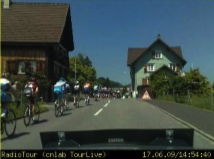
\includegraphics[height=60mm]{images/tourliveweb/tourliveaufnahme.png}
	\caption{Aufnahme aus dem Fahrzeug}
\end{figure}

\subsection{Streckenprofil}
Der Verlauf der Strecke wird in einem Streckenprofil dargestellt. Die Position der Aufnahmegeräte wird mit verschiedenen Farben aufgezeichnet, das Streckenprofil an sich ist statisch und beinhaltet zusätzliche Renn-Informationen wie z.B. Sprints oder Passhöhen. Die Zusatzinformationen und Profildaten werden von Bildern, GPS-Daten und/oder der Marschtabelle übernommen.
\begin{figure}[H]
	\centering
	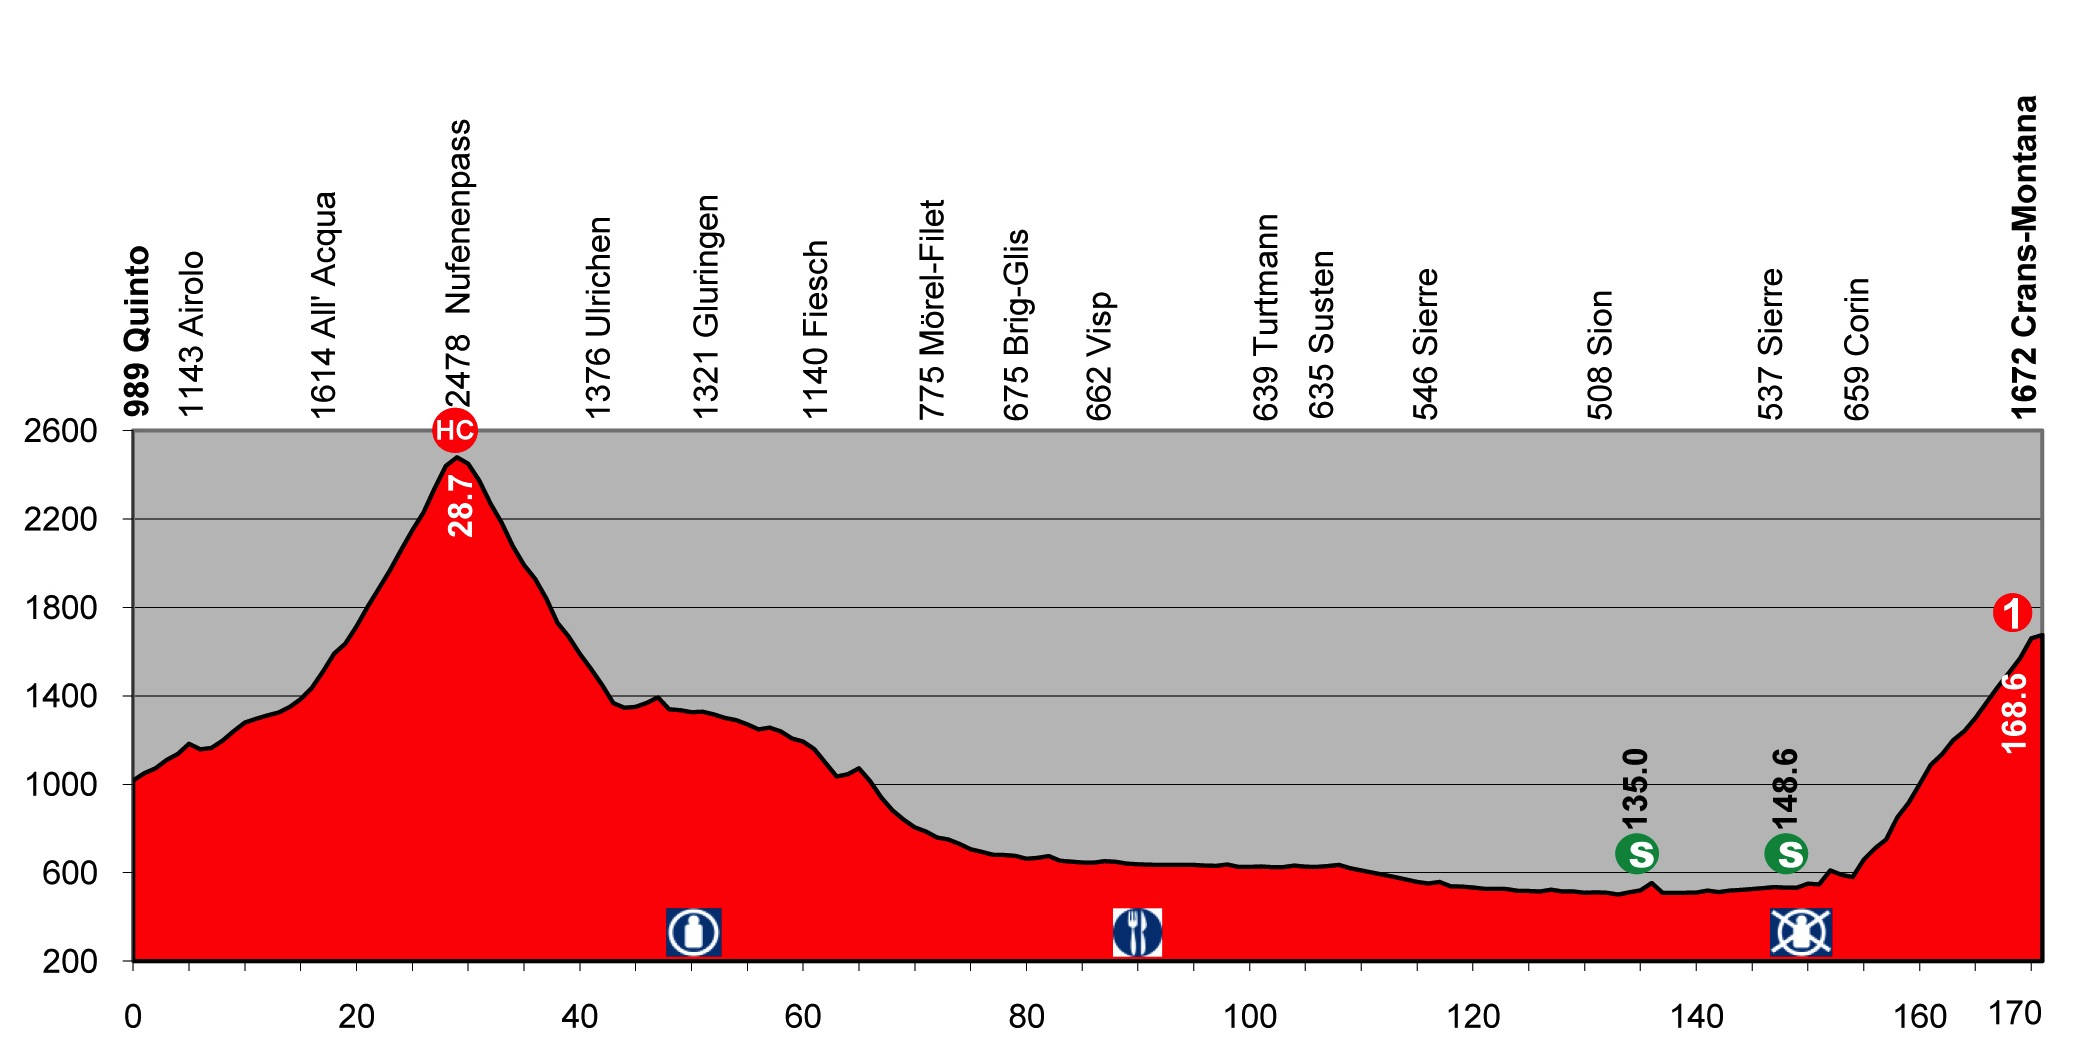
\includegraphics[width=130mm]{images/tourliveweb/streckenprofil.jpg}
	\caption{Streckenprofil aus der Tour de Suisse 2013\footnote{Bildquelle: \url{http://tourdesuisse.ch}, Aufgerufen am 08.05.2013}}
\end{figure}

\subsection{Abstände}
Jedes Aufnahmegerät zeichnet unter anderem die aktuelle Geschwindigkeit auf, diese wird wie in Abbildung 3 dargestellt. Der Server versucht zusätzlich die Distanz zwischen den Geräten zu berechnen und zeigt diese zusammen mit dem zeitlichen Rückstand an. Der TourSpeaker kann zusätzlich den Abstand in der Figur überschreiben, sofern diese Daten aktueller sind
\begin{figure}[H]
	\centering
	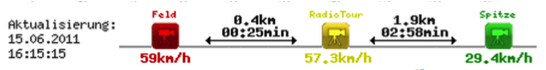
\includegraphics[width=130mm]{images/tourliveweb/abstaende.png}
	\caption{Abstände zwischen den Aufnahmesystemen}
\end{figure}

\subsection{Rennsituation}
Die gegenwärtige Rennsituation wird grafisch dargestellt, bei kleineren (Verfolger-) Gruppen werden die Fahrer namentlich aufgelistet, beim Feld wird nur die gesamte Anzahl Fahrer angezeigt. Der Vorsprung bzw. Rückstand ist bei allen Gruppen relativ zur Spitze angegeben. Zusätzlich wird der letzte Wert ebenfalls angegeben, um eine allfällige Tendenz feststellen zu können.
\begin{figure}[H]
	\centering
	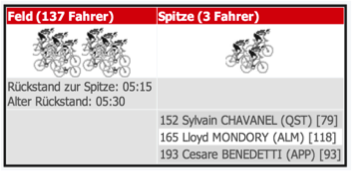
\includegraphics[width=80mm]{images/tourliveweb/rennsituation.png}
	\caption{Die aktuelle Rennsituation dargestellt}
\end{figure}
\subsection{Ranglisten}
Aus der aktuellen Rennsituation lässt sich eine virtuelle (Live) Rangliste bestimmen. Diese Rangliste wiederspiegelt den aktuellen Stand im Rennen, kann beliebig sortiert werden und beinhaltet die folgenden Spalten:
\begin{itemize}
\item Rang
\item Startnummer
\item Fahrername
\item Team
\item Land
\item Rückstand zur Spitze
\end{itemize}
Die offiziellen Ranglisten werden von DataSport / Festina / Matsport bezogen.
\subsection{Kartenausschnitt}
Auf einem Kartenausschnitt wird die zurückgelegte Strecke eingezeichnet, die Positionen der Aufnahmegeräte werden auf der Karte farblich verschieden dargestellt. Die Farben entsprechen den anderen Elementen (siehe Abstände und Stream). Neben Google Maps sollen auch andere Karten-APIs verwendet werden könne
\begin{figure}[H]
	\centering
	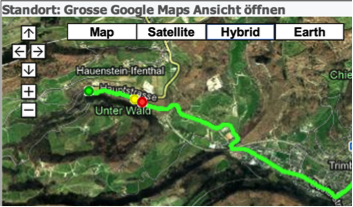
\includegraphics[width=100mm]{images/tourliveweb/kartenausschnitt.png}
	\caption{Die Positionen der Aufnahmegeräte}
\end{figure}
\subsection{Live Ticker}
Eine externe Person kann über ein Webinterface einen Live Ticker führen und Ereignisse während dem Rennen erfassen, diese werden dann sofort auf der Webseite dargestellt.
\subsection{Replay}
Das gesamte Rennen wird aufgezeichnet und kann später in Echtzeit oder im Schnelldurchlauf mit verschiedenen Geschwindigkeiten wiedergegeben werden. Je nach Rennen existieren mehrere Etappen, diese können dann einzeln ausgewählt werden. Die vergangenen Rennen können nach Jahr und Event sortiert und ausgewählt werden.
\subsection{Werbebanner}
Auf der Webseite wird ein Bereich definiert, in welchen Werbebanner dargestellt werden. Diese können in den Einstellungen ein und ausgeschaltet werden.
\subsection{Mobile Version}
Die Webseite soll auch auf Tablets und Smartphones sämtliche Informationen darstellen können. Dabei wird der Ansatz des Responsive Web Design verfolgt wobei die Clients die Webseite entsprechend ihrer Bildschirmgrösse rendern.
\begin{figure}[H]
	\centering 
	
\includegraphics[width=80mm]{images/tourliveweb/responsive.png}
	\caption{Die Darstellung der Webseite auf die Anzeigegrösse angepasst\footnote{Bildquelle:\url{http://johnpolacek.github.com/scrolldeck.js/decks/responsive/img/responsive_web_design.png}, Aufgerufen am 08.05.2013}}
\end{figure}
\subsection{Rennstandort (Marschtabelle)}
Die Besucher der TourLive Webseite können aufgrund Ihres aktuellen Standortes bestimmen, wann die Spitze am jeweiligen Ort eintreffen wird. Der Standort wird durch die Browser Geolocation API ermittelt damit kann dann die Distanz zur Spitze berechnet werden und aufgrund der Durchschnittsgeschwindigkeit den ungefähren Ankunftszeitpunkt.
Die ungefähren Ankunftszeiten gehen auch aus der Marschtabelle hervor. Diese lässt sich ebenfalls anzeigen.

\subsection{Abstandsentwicklung}
Die verschiedenen Aufnahmesysteme können sich unter Umständen weit voneinander entfernen. Die Entwicklung dieses Abstandes während des Rennen bietet für die Radsport-Kenner ein gutes Bild, wie sich das Feld verändert.
\begin{figure}[H]
	\centering
	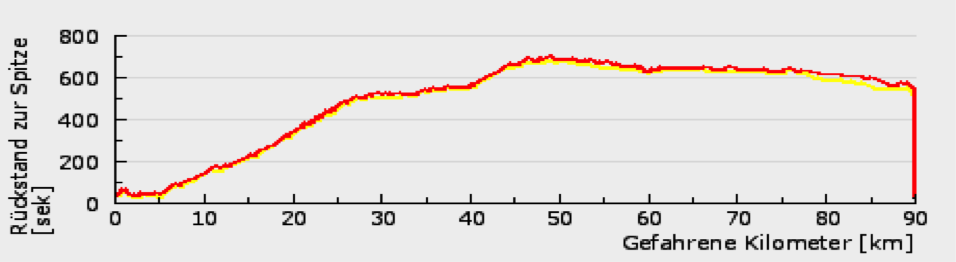
\includegraphics[width=100mm]{images/tourliveweb/abstandsentwicklung.png}
	\caption{Abstandsentwicklung nach Rennkilometer in Sekunden}
\end{figure}

\subsection{Public API}
Sämtliche Grafiken und Daten, welche auf der Webseite angezeigt werden, können auch einzeln über eine festgelegte Schnittstelle als JSON empfangen werden. Dies ermöglicht die Entwicklung von beliebigen Anwendungen durch Dritte. Den Zugang zur öffentlichen Schnittstelle wird durch einen API Key ermöglicht, einen solchen Key erhält, wer sich als Entwickler bei TourLive registriert; dadurch kann die Nutzung überwacht und allenfalls eingeschränkt werden.
\subsection{Input API}
Die aktuelle Rennsituation sowie weitere Informationen zum Rennen werden durch mehrere Android Geräte erfasst. Die Aufnahmegeräte senden sämtliche Informationen via JSON an die Serverschnittstelle. 
\\
Weiter werden Daten direkt vom RadioTour Speaker empfangen, diese liefern vor allem Informationen zur Situation im Rennfeld, wie viele Fahrer in welcher Formation fahren.
\subsection{Nutzungsstatisktik}
Über die Nutzung von TourLive wird eine Statistik geführt. Dabei wird auf eine bestehendes Web Analytics System zurückgegriffen, dieses System ist nicht Bestandteil der Arbeit es wird dabei auf Piwik oder Google verwendet.
\newpage
\section{Anforderungen Android und Device Management Server}
\label{sec:anforderungenandroiddevmgmt}

\subsection{Funktionsumfang bestehendes Aufnahmesystem}
Das bestehende TourLive System basiert auf einer Symbian App, die über Nokia Modelle (z.B. Nokia N82 und Nokia X6) betrieben werden. Die Daten (Positionsdaten, Bilder, Videostream) werden über das Mobilfunknetz via ein proprietäres Protokoll zum bestehenden TourLive-Server übertragen. Über eine Gerätestatusseite\footnote{bisherige Gerätestatusseite, \url{http://www.tourlive.ch/tds12/status.php}, aufgerufen am 27.02.2013}   können einfache Geräteverwaltungsaufgaben durchgeführt werden. Folgende Übersicht bietet einen groben Überblick über das aktuelle System: \url{
http://www.cnlab.ch/tourlive/Radrennen.html#TourLive_Aufnahmesysteme_im_Tour_Tross} \\

Das Symbian System soll nun auf Android portiert werden, wobei der Funktionsumfang für den ausschliesslichen Einsatz bei Radrennen eingegrenzt wird. 

\subsubsection{Views}
Die aktuelle Symbian App bietet folgende Views. Diese werden in 3 Spalten beschrieben, wobei die rechte Spalte einen Ausblick in die neue Android App und deren Funktionalität darstellt. Die Angaben unter „Neues System“ dienen jedoch nur der Übersicht und im Vergleich zum alten System. Eine exakte Spezifizierung inklusive neuer Funktionalitäten erfolgt im nächsten Kapitel.

Diese View wird beim Start der App angezeigt. Über die beiden Pfeile in der horizontalen Navigationsleiste wird über die verschiedenen Views navigiert.

\begin{longtable}{p{4.5cm} p{3cm} p{4.5cm}}
\textbf{Altes System - View GPS Info}
	\begin{itemize}	[noitemsep,nolistsep] 
		\item Geschwindigkeit [km/h]
		\item Höhe [m]
		\item Richtung (in Azimut) / Beschleunigung (Beschleunigung kann weggelassen werden)
		\item Steigung [\%]
		\item Latitude (Koordinate)
		\item Longitude (Koordinate)	 
	\end{itemize} 
	
	&   \raisebox{-\totalheight}{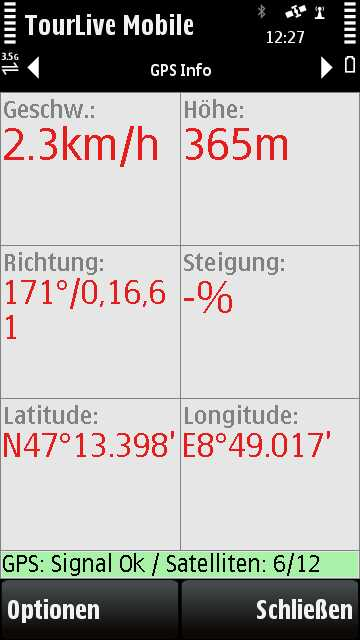
\includegraphics[width=3cm]{images/android/screensnap/GPSInfo.jpg}}
	& \textbf{Neues System} \newline
	\begin{itemize}		[noitemsep,nolistsep] 
		\item Geschwindigkeit [km/h]
		\item Höhe [m]
		\item Richtung (in Azimut) 
		\item Steigung [\%], über 100m gerechnet
		\item Latitude (Koordinate)
		\item Longitude (Koordinate)	
	\end{itemize}\\


	\textbf{Altes System - View Trip Info}  \newline
	View erreichbar durch einfaches Betätigen der „nach links“-Navigation.  	\begin{itemize}	[noitemsep,nolistsep] 
		\item Zeit Trip [hh:mm:ss]
		\item Höhe Trip [m]
		\item Distanz [km]
		\item Durchschnittliche Geschwindigkeit [km/h]
		\item UTC Zeit (Weltzeit)
		\item Datum (aktuelles Datum)
	\end{itemize}
	&   \raisebox{-\totalheight}{ 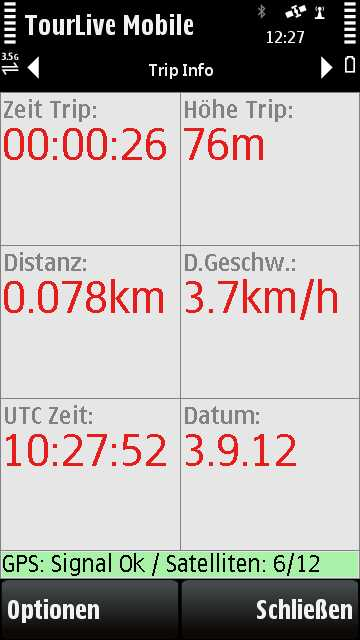
\includegraphics[width=3cm]{images/android/screensnap/TripInfo.jpg}  }
 	& \textbf{Neues System}\newline
	\begin{itemize}	[noitemsep,nolistsep]
		\item Zeit [hh:mm:ss]
		\item Höhe [m]
		\item Distanz [km]
		\item Durchschnittliche Geschwindigkeit [km/h]
	\end{itemize}\\

	\textbf{Altes System - View Total Info} \newline
	View erreichbar durch zweifaches Betätigen der „nach links“-Navigation.  
	\begin{itemize}[noitemsep,nolistsep]
		\item Zeit Total [hh:mm:ss]
		\item Zeit Tour [hh:mm:ss]
		\item Distanz Total [km]
		\item Distanz Tour [km]
		\item Höhe Total [m]
		\item Höhe Tour [m]
	\end{itemize} 
	&   \raisebox{-\totalheight}{ 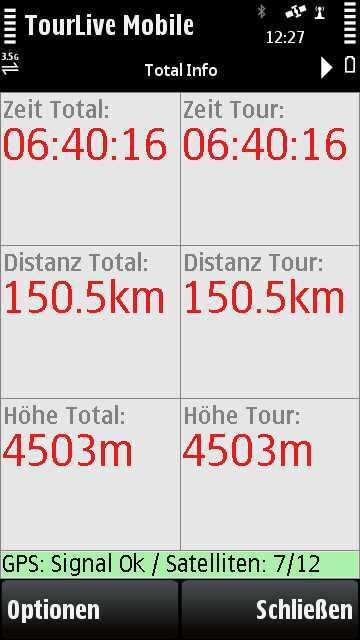
\includegraphics[width=3cm]{images/android/screensnap/TotalInfo.jpg}  }
	& \textbf{Neues System} \newline
	Diese View fällt weg. Es werden nur noch Daten pro Etappe erfasst. \\
	

	\textbf{Altes System -  View ODB Info} \newline 
	View erreichbar durch einfaches Betätigen der „nach rechts“-Navigation.    \newline
On Board Diagnose Bus (war für Benzinverbrauch, Motordrehzahl)	Bezieht sich auf ein externes Gerät. Ist im neuen System irrelevant und wird deshalb an dieser Stelle nicht dokumentiert. \newline 
	& \newline \newline Bezieht sich auf ein externes Gerät. Ist im neuen System irrelevant und wird deshalb an dieser Stelle nicht dokumentiert.  
	&\textbf{Neues System} \newline \newline 
Diese View fällt weg. Ein OBD wird nicht mehr benötigt. \\
	
	\textbf{Altes System -   View ODB Verbrauch} \newline 
	iew erreichbar durch zweifaches Betätigen der „nach links“-Navigation. 
	& \newline \newline Bezieht sich auf ein externes Gerät. Ist im neuen System irrelevant und wird deshalb an dieser Stelle nicht dokumentiert. \newline
	&\textbf{Neues System} \newline \newline 
Diese View fällt weg. \\
	
	\textbf{Altes System -  View Puls Info} \newline  
	View erreichbar durch dreifaches Betätigen der „nach links“-Navigation. \newline
On Board Diagnose Bus (war für Benzinverbrauch, Motordrehzahl)	Bezieht sich auf ein externes Gerät. Ist im neuen System irrelevant und wird deshalb an dieser Stelle nicht dokumentiert. \newline 
	& \newline \newline Bezieht sich auf ein externes Gerät. Ist im neuen System irrelevant und wird deshalb an dieser Stelle nicht dokumentiert.  
	&\textbf{Neues System} \newline \newline 
Diese View fällt weg. Ein OBD wird nicht mehr benötigt.\\
	
	\textbf{Altes System -   View ODB Verbrauch} \newline 
	iew erreichbar durch zweifaches Betätigen der „nach links“-Navigation. 
	& \newline \newline Bezieht sich auf ein externes Gerät. Ist im neuen System irrelevant und wird deshalb an dieser Stelle nicht dokumentiert.
	&\textbf{Neues System} \newline \newline 
Diese View fällt weg. Ein externes Puls Messgerät wird nicht mehr benötigt.\\


	\textbf{Altes System - View Netz Info}  \newline
	View erreichbar durch vierfaches Betätigen der „nach links“-Navigation.  
	\begin{itemize}[noitemsep,nolistsep]
		\item Zellen ID (Funkzellen Nummer)
		\item Area (Location Area)
		\item Signal (Signalstärke in dB)
		\item Akku (Akku Ladestatus)
		\item Netzwerk (Provider) 
		\item Netzwerk ID (Verbindungseigenschaften) \newline
		228 = Mobile Network Code \newline
		01 = Mobile Country Code \newline
		UMTS = Technologie
	\end{itemize}
	&   \raisebox{-\totalheight}{ 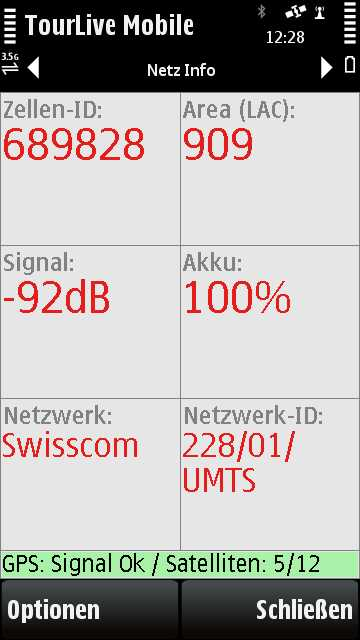
\includegraphics[width=3cm]{images/android/screensnap/NetzInfo.jpg}  }
 	& \textbf{Neues System} 
	\begin{itemize}	[noitemsep,nolistsep]
		\item Zellen ID
		\item Area
		\item Signal
		\item Netzwerk ID
		\item Technologie (UMTS) 
		\item Datenrate \newline
	\end{itemize}
		\textbf{Zusätzlich}
	\begin{itemize}	[noitemsep,nolistsep]
		\item RTT
		\item Packet-Loss
	\end{itemize}\\


	\textbf{Altes System - View Logs}  \newline
View erreichbar durch fünffaches Betätigen der „nach links“-Navigation.   \newline
Log um Fehlerquellen zu eruieren. \newline

	&   \raisebox{-\totalheight}{ 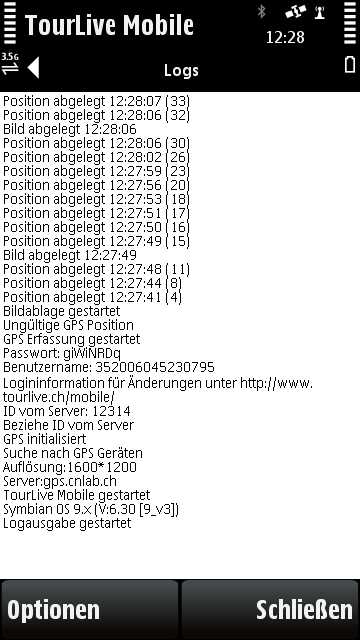
\includegraphics[width=3cm]{images/android/screensnap/Logs.jpg}  }
 	& \textbf{Neues System} \newline 
	Diese View wird in einem ähnlichen Stil beibehalten.\\


	\textbf{Altes System - View Hauptmenü}  \newline
	View wird sichtbar durch das Betätigen des „Optionen“-Buttons.
	\begin{itemize}[noitemsep,nolistsep]
		\item Start der Aufzeichnung
		\item Konfiguration der App (siehe unten)
		\item Bild auslösen (manuelle Bildauslösung)
		\item Hintergrundbe- leuchtung (Ein / Ausschalten > Stromsparfunktion)
		\item ODB > nicht mehr relevant
		\item Puls > nicht mehr Relevant
		\item GPS [Submenü]
		\item Reset GPS Trip Daten
		\item Reset GPS Tour Daten
		\item Reset alle GPS Daten
	\end{itemize}
	&   \raisebox{-\totalheight}{ 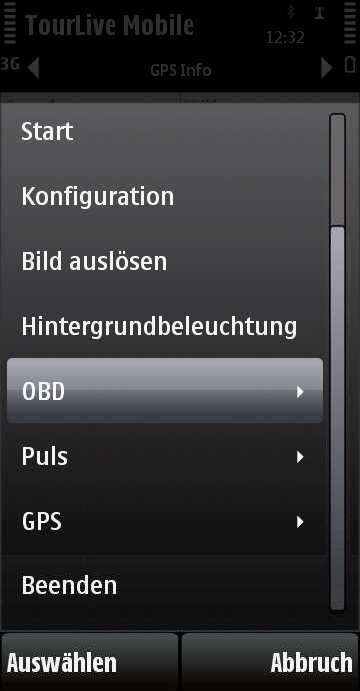
\includegraphics[width=3cm]{images/android/screensnap/Hauptmenue_1.jpg}  }
 	& \textbf{Neues System} \newline
	\begin{itemize}[noitemsep,nolistsep] 
		\item Einstellungen
		\item About
	\end{itemize}\\


	\textbf{Altes System - View Konfiguration}  \newline
	View wird sichtbar durch das Betätigen des „Konfiguration“-Buttons im Optionen-Menü.
	\begin{itemize}[noitemsep,nolistsep]
		\item Benutzername
		\item Grösse (irrelevant in der neuen Version)
		\item Gewicht (irrelevant in der neuen Version)
		\item Alter (irrelevant in der neuen Version)
		\item Geschlecht (irrelevant in der neuen Version)
		\item GPS Intervall (0 – 600 sec)
		\item GPS Speichern Intervall (0 – 600 sec)
		
	\end{itemize}
	&   \raisebox{-\totalheight}{ 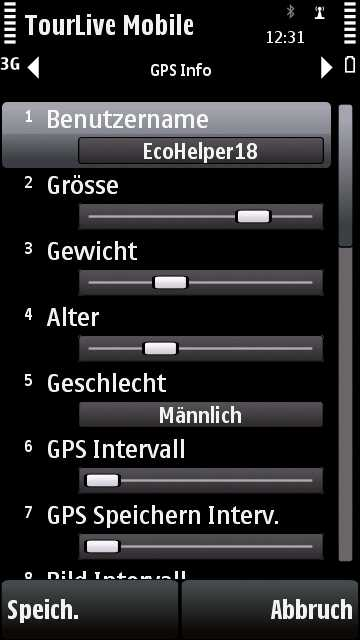
\includegraphics[width=3cm]{images/android/screensnap/Konfiguration_1.jpg}  }
 	& \textbf{Neues System} \newline
	\begin{itemize}	[noitemsep,nolistsep]
		\item Benutzername
		\item GPS Intervall (0 – 60 sec)
		\item GPS Speichern Intervall (0 – 600 sec) (Wird mit GPS Intervall zusammengefasst)
		\item Bild Intervall (0 – 60 sec)
		
	\end{itemize}
	\\

	\begin{itemize}[noitemsep,nolistsep]
		\item Bild Intervall  (0 – 600 sec)
		\item Einheiten (km – Meilen - ..) (nur noch MKS Einheiten standardmässig)
		\item Zusatzgerät (irrelevant in der neuen Version)
		\item Video Streaming (Ein / Aus)
		\item Bilder drehen (Ein / Aus)
		\item Offline Mode (Ein / Aus) (irrelevant in der neuen Version, wird automatisch gemacht)
		\item GPS Dateiformat (TourLive + Google Earth, Google Earth) (irrelevant in der neuen Version, wird serverseitig gerechnet)
	\end{itemize}
	&  \raisebox{-\totalheight}{ 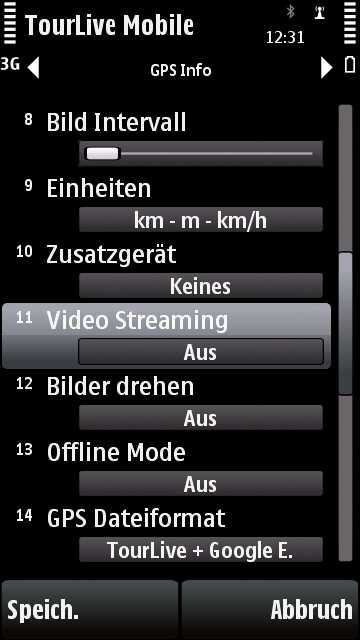
\includegraphics[width=3cm]{images/android/screensnap/Konfiguration_2.jpg}  } 
 	& 
	\begin{itemize}	[noitemsep,nolistsep]
		\item Bild Intervall (0 – 60 sec)
		\item Video Streaming (Ein / Aus)
		\item Bilder drehen (Ein / Aus)
		\item Automatischer Start (Neu verschiedene Modi)
		\item Hintergrundbeleuchtung (Normal / Dauernd an)
		\item Bildauflösung
		\item Bildmodus
	\end{itemize}\\

\begin{itemize}[noitemsep,nolistsep]
\item Automatischer Start (Ein / Aus)
\item Hintergrundbe- leuchtung (Normal / Dauernd an)
\item Einfaches Beenden (Ein / Aus) (irrelevant in der neuen Version)
\item Schreibe Logfile (Ein / Aus) (irrelevant in der neuen Version, wird immer geschrieben)
\item Heartbeat Ton (Lautstärke) (irrelevant in der neuen Version, keine Töne mehr)
\item Fehlerton (Lautstärke) (irrelevant in der neuen Version, keine Töne mehr)
\item Bildauflösung (1600 x 1200 , …)
\item Bildmodus (Portrait / Landscape)

\end{itemize}
	&  \raisebox{-\totalheight}{ 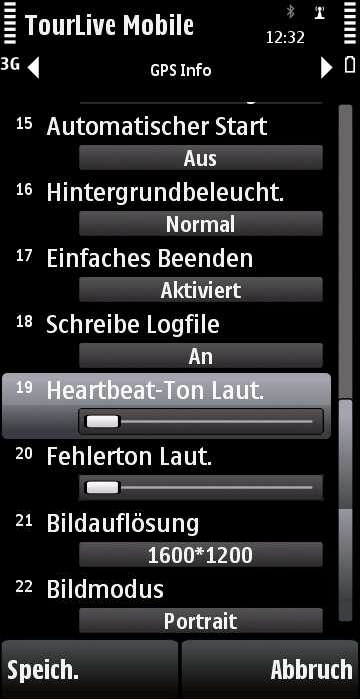
\includegraphics[width=3cm]{images/android/screensnap/Konfiguration_3and4_combined.jpg}  } 
 	& 
	\textbf{Zusätzlich} 
	 \begin{itemize}[noitemsep,nolistsep]
		\item Kritischer Akkustand
		\item Betriebsmodus
		\item TourLive Server Primär
		\item TourLive Server Sekundär
		\item Device Management Server
		\item Kamera automatisch ausrichten
		\item Videoauflösung
		\item Renndistanz Korrektur
		\item Gespeicherte Daten löschen
	\end{itemize}\\

\end{longtable}
 


\subsection{Anforderungen – Neues Aufnahmesystem}
Das neu zu entwickelnde Aufnahmesystem basiert grundsätzlich auf der Funktionalität der  bestehenden Symbian App. Wobei auf die Unterstützung  externer Geräte (Puls-Messung, Onboard Diagnose Bus (OBD)), verzichtet werden kann. Einen Überblick über die übernommenen Funktionen bietet die dreispaltige Beschreibung im Kapitel „Funktionsumfang bestehendes Aufnahmesystem [Symbian App]“.

\subsubsection{Hardware / Software - Aufnahmesystem}
Bei den Aufnahmegeräten wird gemäss Vorgabe des Auftraggebers auf das Betriebssystem Android ab Version 4.x (Ice Cream Sandwich) gesetzt. Der Prototyp wird auf zwei Samsung Nexus Geräten getestet. Mittelfristig soll die zu entwickelnde App auf Geräten von verschiedenen Herstellern (Samsung, HTC, ...) betrieben werden können. Im Rahmen der Arbeit ist die App auf zwei bis drei weiteren Geräten zu testen.
\subsubsection{Betriebsmodi / Device Management}
Die Geräte sollen sowohl über ein Management-Portal, analog zum zur bisherigen Verwaltungsseite \footnote{Verwaltungsseite, \url{http://www.tourlive.ch/tds11/status.php}, aufgerufen am 27.02.2013} , fernverwaltet als auch über ein „Einstellungen“-Menü direkt am Gerät konfiguriert werden können. \\

Daraus resultieren zwei Betriebsmodi: „managed“ und „unmanaged“. Beim ersten App-Start nach der Installation der App, wird der Benutzer gefragt, in welchem Modus das Aufnahmesystem betrieben werden soll. Die beiden Modi lassen sich am Gerät selber jederzeit ändern. Wählt der Benutzer beim ersten App-Start innerhalb von 10 Sekunden keinen Modus, wird das Gerät automatisch in den Betriebsmodus „managed“ versetzt und eine Standardkonfiguration vom Device Management Server bezogen.\\

Bei allen weiteren App-Starts werden die Einstellungen vom letzten Betrieb übernommen sofern der Betriebsmodus zuvor „unmanaged“ war. War der Betriebsmodus auf „managed“ eingestellt, so wird die Konfiguration vom Management Server bezogen. Ist dieser nicht verfügbar, wird der Modus auf „unmanaged“ gesetzt und die existierenden Einstellungen verwendet.
\paragraph{Device Management Portal}
Über das Management-Portal können Geräteprofile beziehungsweise ein Standardprofil definiert werden, die bei Verwendung des „managed“ – Modus verwendet werden. Die Geräte werden über eine eindeutige Identifikationsnummer identifiziert.
Ebenfalls Bestandteil des Management-Portals ist Einsicht bzw. Abrufen der Applikationslogs zur Eruierung allfälliger Fehlerquellen. Das Applikationslog soll jedoch auch direkt am Gerät eingesehen und mit den üblichen Android „Share“-Optionen (z.Bsp.: Versand per E-Mail,...) geteilt werden können.
\subparagraph{Betriebsmodus „managed“}
Der Betriebsmodus „managed“ erlaubt eine vollständige Fernverwaltung der Android App. Wird das Gerät eingeschaltet, bezieht es vom Device Management Server eine App-Konfiguration. Sämtliche Einstellungen werden über das Managementportal vorgenommen. Am Gerät selber können keine Einstellungen mehr vorgenommen werden. Die Einstellungen werden als read-only angezeigt. Es ist am Gerät jedoch möglich, den Betriebsmodus zu ändern.
\subparagraph{Betriebsmodus „unmanaged“}
Der Betriebsmodus „unmanaged“ funktioniert genau umgekehrt. Die Einstellungen des Gerätes werden zwar auf dem Device-Management-Server angezeigt, können jedoch nicht verändert werden. Die Einstellungen werden lokal am Gerät vorgenommen.  Über das Device Management Portal ist es jedoch möglich, den Betriebsmodus zu ändern
\paragraph{Notfallwiederherstellung}
Über einen weiteren Management-Kanal (z.Bsp.: SMS) soll eine Notfallwiederherstellung des Systems ermöglicht werden. Beispielsweise wenn das Gerät über das Mobilfunkdatennetz nicht mehr erreichbar ist. Dieser Notfallwiederherstellungsservice wird ein eine Zweit-App ausgegliedert, damit beim Crash der Haupt-App zumindest der Notfallwiederherstellungsservice noch funktioniert.
\paragraph{Betriebslog}
Geloggt wird unter anderem folgendes:
\begin{itemize}
\item ganze Kommunikation mit dem Server
\item Aufnahme Start/Stop
\item Exceptions
\end{itemize}


\subsubsection{Funktionalität TourLive App}
\paragraph{Allgemein}
Die nachfolgend beschriebenen Daten die gesammelt werden (Bilder, Positionen, etc.) werden einem Rennen bzw. einer Etappe zugeordnet. Eine Etappe (z.Bsp.: Etappe 1 des Rennens Tour de Suisse) ist einem Rennen (z.Bsp. Tour de Suisse) zugeordnet. Es gibt Rennen, welche nur eine Etappe haben. Dies als Einführung ins Gesamtsystem. Am Aufnahmesystem beziehungsweise in der Android-App ist es nicht möglich Rennen oder Etappen zu definieren. Die gesammelten Daten werden versehen mit einem Zeitstempel und einer eindeutigen Geräteidentifikationsnummer an den TourLiveServer gesendet. Das matching zum entsprechenden Rennen beziehungsweise der Etappe erfolgt erst auf dem Server. \\

Zur Aufnahme  und Übertragung der Daten werden vier verschiedene Aufnahmestart-Modi unterschieden:
\begin{itemize}
	\item Manuell (direkt über den Hauptscreen der App)
	\item Zeitbasiert
	\item Fernverwaltung (start über das Device Management Portal)
	\item Bei Aktivierung einer externen Stromquelle (Feuerzeuganzünder im Auto,..)
\end{itemize}

\paragraph{Positionsaufnahme}
Die primäre Funktion des Aufnahmesystems besteht in der Aufnahme von Geopositionsdaten, deren Weiterverarbeitung und der Übermittlung an den TourLive-Server. Über das GPS-Modul des Mobilfunkgerätes werden folgende Daten ermittelt:
\begin{itemize}
\item Aktuelle Position [GPS Longitude / Latitude]
\item Aktuelle Höhe (GPS Höhe) [m]
\item Aktuelle Zeit (GPS Timestamp) [unix\_time]
\item Geschwindigkeit (wird gelesen) [km/h]
\item Richtung (in Azimut, wird berechnet) [°]
\item Steigung (über die letzten 100m, wird berechnet) [\%]
\item Anzahl Satelliten mit denen das Aufnahmegerät verbunden ist
\end{itemize}
Für die Aufzeichnung der Positionsdaten per GPS stehen folgende Einstellungen zur Wahl:
\begin{itemize}
\item Aufnahmeintervall der Positionsdaten (1, 2, 5, 10, 15, 30, 60 sec)
\end{itemize}

\paragraph{Bildaufnahme}
Ein wesentlicher Bestandteil des Aufnahmesystems ist die Übertragung von Bildmaterial in Form von einzelnen Bildern oder einem Videostream. Folgende Funktionalität muss dabei beachtet werden:
\begin{itemize}
\item Anpassung der Bildauflösung adaptiv an die verfügbare Datenraten (optional)
\item Bilder sollen automatisch, in der korrekten Ausrichtung an den Server geschickt werden (Stichwort Gerätesensoren)
\end{itemize}

Desweitern sollen bezüglich Bildaufnahme verschiedene Einstellungen zur Auswahl stehen:
\begin{itemize}
\item Einzelbilder mit konfigurierbaren Aufnahmeintervallen (1, 2, 5, 10, 15, 30, 60 sec)
\item Videostream (echter Videostream oder schnelles Aneinanderreihen von Einzelbildern)
\item Front-/Back-Kamera muss wählbar sein
\end{itemize}
	
\paragraph{Power Management}
Während der Tour wird das Aufnahmegerät über den Zigarettenanzünder mit Strom versorgt. Fällt diese Stromversorgung aus beziehungsweise fällt der Akku-Stand unter einen kritischen Grenzwert, so soll ein Energiesparmodus aktiviert werden um das Aufnahmesystem möglichst lange Betriebsbereit zu halten. Dieser Stromsparmodus umfasst:
\begin{itemize}
\item Vergrösserung GPS-Intervall
\item Verkleinerung Bild-Auflösung (weniger Daten müssen übertragen werden)
\item Vergrösserung Daten-Übertragungs-Intervall an TourLive Server (Overhead wird gespart)
\item Deaktivierung Video-Streaming
\item Herunterfahren der Bildschirmhelligkeit
\end{itemize}

\label{par:alarming}
\paragraph{Alarming Funktionen}
Treten Probleme auf, so soll auf dem Telefon sowie in der Management Konsole darüber informiert werden. Als zu meldende Probleme gelten folgende:
\begin{itemize}
\item GPS nicht verfügbar oder zu wenig Satelliten
\item Keine Mobile-Verbindung 2 Minuten
\item Smartphone wird nicht mehr geladen (Stromzufuhr unterbrochen)
\item Smartphone Akkustand ist unter 50\%, 25\%, 10\%
\end{itemize}

	
\paragraph{Kommunikation mit dem TourLive Server}
Die gesammelten Textdaten werden über eine offene, freie Schnittstelle (z.Bsp. \textit{\gls{http}}/\textit{\gls{json}}) an einen Webservice (TourLive Server) übertragen. Eine ähnliche Lösung soll für das Bildmaterial sowie für den Videostream gefunden werden.

\paragraph{Kommunikation mit dem Device-Management Server}
Die Kommunikation mit dem Device-Management Server erfolgt ebenfalls über eine offene, freie Schnittstelle. Zusätzlich soll die Möglichkeit einer Notfallwiederherstellung über einen Drittkanal (z.Bsp.: SMS) realisiert werden.

\paragraph{Mobile Performance Informationen}
Die Streckenführung der Tour de Suisse wird jedes Jahr neu festgelegt. Dabei  wird selbstverständlich keine Rücksicht auf die Netzabdeckung der Mobilfunknetze genommen. Gerade bei Bergetappen abseits der Zivilisation muss mit einer mässigen Netzabdeckung gerechnet werden. Die Analyse der Verbindungseigenschaften (Packet Loss, RTT,..) soll Aufschluss darüber bringen, wann und wo keine Daten übertragen werden konnten und dient somit einer allfälligen Fehleranalyse. Konkret sollen folgende Daten erfasst werden:
\begin{itemize}
\item Zellennummer (Mobilfunkantenne)
\item Location Area Code (LAC)
\item Mobile Netzwerk Code (MNC) (Provider)
\item Mobile Country Code (MCC)
\item Signal (Signalstärke in dB) und/oder „Striche“
\item Übertragungsstandard [GPRS, EDGE, UMTS, LTE,..])
\item Download Datenrate
\item Upload Datenrate
\item RTT
\item Packet Loss (Dup Acks)
\end{itemize}
	
\subsection{Nichtfunktionale Anforderungen}
Neben der effektiven App-Funktionalität müssen folgende nichtfunktionalen Anforderungen beachtet werden.
\subsubsection{Sicherheit}
In Bezug auf Vertraulichkeit und Integrität werden keine speziellen Anforderungen gestellt. Die Datenübertragung erfolgt unverschlüsselt. Das Aufnahmegerät muss sich am TourLive Server nicht explizit authentisieren. In Bezug auf Verfügbarkeit sind die Anforderungen hoch. Während dem Rennen soll es keine Lücken ohne Daten von mehr als 5 Minuten geben. Können während einer bestimmten Zeitspanne keine Daten übertragen werden, sollen diese gepuffert und zu einem späteren Zeitpunkt übertragen werden. 
\paragraph{Ausfallsicherheit}
Die gesammelten Daten (Positionen, Bilder,..) werden parallel auf dem lokalen Gerätespeicher abgelegt. Erreicht dieser 80\% der verfügbaren Kapazität werden automatisch alte Eventdaten gelöscht. Über dieses lokale Caching wird sichergestellt, dass die  gesammelten Daten aufgrund technischer Probleme bei der Datenübertragung nicht verloren gehen. 
\subsubsection{Anforderungen ans GUI}
Das GUI soll intuitiv ohne Anleitung oder Einführung bedient werden können. 
\paragraph{Mehrsprachigkeit}
In der Grundversion werden die Sprachen Deutsch und Englisch unterstützt. In einem späteren Schritt soll man die Möglichkeit haben, die App um weitere Sprachen einfach zu ergänzen.


\section{Evaluation Webframework}
\label{sec:evaluationwebframework}
\subsection{Kriterienkatalog}
Die folgende Kriterien wurden zusammen mit dem Industriepartner definiert und festgelegt:
\begin{itemize}
\item Open Source Software, keine Lizenzgebühren
\item Beispiel- und Referenzprojekte vorhanden
\item Hohe Performance und stabile Verfügbarkeit auch bei hoher Auslastung
\item Skalierbar für mehrere Rennen und Etappen
\item Datenbankanbindung an \textit{\gls{mariadb}}
\item Weiterentwicklung durch cnlab AG muss möglich sein
\end{itemize}
Optionale, gewünschte Anforderungen:
\begin{itemize}
\item Vorkenntnisse in der betreffenden Programmiersprache
\item Gleiche Technologie für \textit{\gls{api}}, Webseite und Datenverarbeitung
\item Umfangreiche Dokumentation und Tutorials (Community\footnote{Die Community ist die Verbreitung einer Technologie sowie die Hilfsbereitschaft in Foren und Portalen. Dies ist äusserts schwierig zu beurteilen und kann sich auch schnell ändern.})
\end{itemize}
\subsection{Mögliche Lösungen}
\subsubsection{Django}
Django ist ein auf Python basiertes Webframework. Es wird eingesetzt bei berühmten Webseiten wie z.B. Pinterest, Instagram und The Washington Post.  Django beinhaltet einen OR Mapper, Templates zur Darstellung und einen URL Dispatcher als Controller.
\subsubsection{Spring MVC}
Spring MVC ist ein Framework für die Erstellung von Webprojekten. Es basiert auf Java Technologien und fördert Dependency Injection  und aspektorientierte Programmierung.
\subsubsection{JavaServer Faces}
JSF ist ein Framework-Standard für Webapplikationen in Java. Es verwendet die Java Servlet Technologie und benötigt einen Servlet Container für den Betrieb. Mit JSF können Komponenten für User Interfaces einfach in Webseiten eingebaut werden. 
\subsubsection{Symfony}
Symfony ist ein Open Source PHP Webframework und verfolgt das MVC Pattern. Die Zuordnung der Models geschieht dabei über die Namensgleichheit in Singular und Plural und nicht über Konfigurationsdateien (convention over configuration). Weiter können durch Konsolenapplikationen Anwendungen generiert werden.
\subsubsection{Ruby on Rails}
Rails ist ein Webframework geschrieben in Ruby. Es ist geprägt von den Prinzipien „don’t repeat yourself“ und „convention over configuration“. Ruby on Rails besteht aus fünf Modulen, jedes dieser Module übernimmt gewisse Funktionen, so z.B. der Action Mailer versendet und empfängt E-Mails.
\subsection{Nutzwertanalyse}
\begin{figure}[H]
	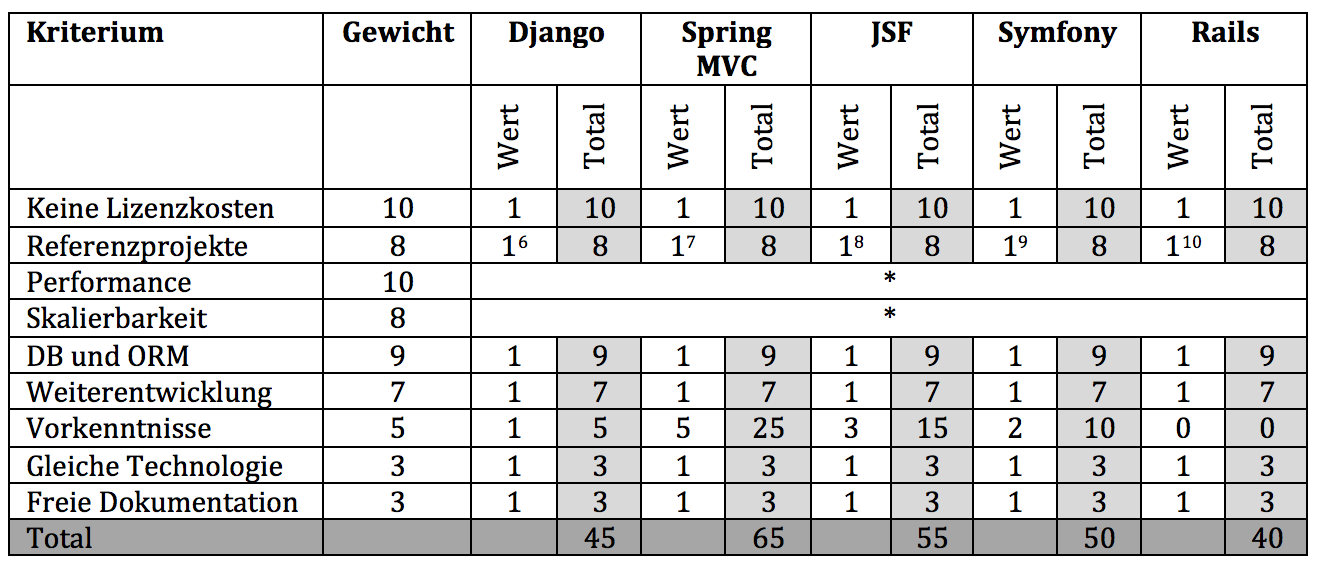
\includegraphics[width=130mm]{images/tourliveweb/nutzwertanalyse.png}
	\caption{Nutzwertanalyse}
\end{figure}
\subsubsection{Erläuterung zu Performance und Skalierbarkeit}
Bezüglich der Performance gibt es verschiedene Ansichten zu den verschiedenen Frameworks. Da es aber zu allen obigen Frameworks grosse Projekte gibt, kann davon ausgegangen werden, dass die Performance und Skalierbarkeit für das TourLive Projekt ausreicht.
\subsubsection{Erläuterung zur Gewichtung der Kriterien}
Die verschiedenen Kriterien wurden in einer Skala von 1 – 10 gewichtet, wobei 10 das wichtigste Kriterium darstellt. Gemäss cnlab Software AG dürfen für das Framework keine Lizenzkosten anfallen und die Webseite muss auch unter Last stabil verfügbar sein. Daher werden diese beiden Kriterien mit dem höchsten Gewicht 10 versehen.
Da das System einen stark wachsenden Datenbestand haben wird, ist die Implementation von Datenbanken ebenfalls von grosser Bedeutung. Referenzprojekte dienen als Beweis für die Skalierbarkeit und die Performance des jeweiligen Frameworks.
Für die Studierenden ist der Zugang zu freier Dokumentation sowie Vorkenntnisse relevant, jedoch nicht zwingend erforderlich. Wünschenswert ist ebenfalls, dass für das gesamte Webprojekt dasselbe Framework verwendet werden kann. Diese Punkte werden daher mit den Gewichten 3-5 bewertet.
\subsubsection{DB und ORM}
Ruby on Rails verfolgt das Ziel möglichst abstrakt mit Datenbanken zu arbeiten und kann deshalb problemlos mit verschiedenen Datenbanksystemen arbeiten. Gleiches gilt für den Ansatz bei Django, dort werden verschiedene Datenbankadapter zur Verfügung gestellt. Auch Spring arbeitet z.B. mit Hibernate als ORM problemlos mit verschiedenen Datenbanken.
\subsubsection{Weiterentwicklung durch cnlab Software AG}
Nach Abschluss der Arbeit wird das Projekt durch die cnlab weiterentwickelt. Daher muss bei der Auswahl des Frameworks darauf geachtet werden, dass eine weitere Entwicklung möglich ist.
\subsubsection{Schlussfolgerungen}
Da die Frameworks sehr ähnliche Ansätze verfolgen und aktuell eine grosse Entwicklergemeinschaft geniessen, sind die Unterschiede, abgesehen von der Programmiersprache welche als Grundlage dient, sehr klein. Entscheidend sind schliesslich die Vorkenntnisse: Java ist diejenige, für die bereits das grösste Vorwissen besteht. Daher sind für die engere Wahl die beiden Lösungen Spring MVC und JSF im Rennen. Da wir in einer kleinen Projektarbeit bereits mit JSF gearbeitet haben, möchten wir nach unseren eher negativen Erfahrungen damit von einer Entwicklung mit JSF absehen und auf das Spring MVC Framework setzen.

\subsection{Anmerkung zum Framework}
Das Java Spring MVC Webframework baut auf dem Prinzip \textit{Dependency Injection} auf. Dependency Injection wird unter anderem mit dem Begriff Inversion of Control zusammengefasst und im folgenden Abschnitt erläutert. Weiter fördert Spring gute Programmierpraktiken wie z.B. die Trennung von Model, View und Controller oder die Verwendung von Objekt relationalen Mappern beim Einsatz von Datenbanken in der Persitenzschicht.

\subsubsection{Dependency Injection}
Die Grundlage für Dependency Injection basiert auf dem Prinzip, dass möglichst wenig Abhängigkeiten eines Objekts von einem anderen Objekt besitzt werden. Die Abhängigkeiten sollen zur Verfügung gestellt werden. So kann unabhängig von der Implementation auf die Schnittstellen zugegriffen werden. Dies erlaubt zum Beispiel einen späteren Austausch der Abhängigkeit. In Spring übernimmt der Dependency Injection Container diese Aufgabe. Die benötigten Abhängigkeiten können entweder mit einer Annotation im Code oder durch Konfiguration in einer xml Datei deklariert werden. Die nachfolgende Grafik stammt von Martin Fowlers Artiekel zum Thema Dependency Injection \cite{martinfowler2004}.
\begin{figure}[H]
	\centering
	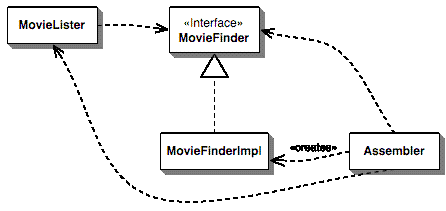
\includegraphics[width=100mm]{images/tourliveweb/dependencyinjection.png}
	\caption{Dependency Injection nach Martin Fowler \cite{martinfowler2004}}
	\label{fig:dpendencyinjection}
\end{figure}
Die Funktionsweise kann am einfachsten anhand des Beispiels von Martin Fowler in Abbildung \ref{fig:dpendencyinjection} aufgezeigt werden. Die Klasse MovieLister zeigt und filtert Filme. Dabei spielt die Quelle woher die Filme kommen keine Rolle. MovieLister benötigt nur eine Liste von Filmen (Abhängigkeit). Die MovieFinderImpl Klasse bietet genau diese Möglichkeit und zeigt dies durch die Implementation des MovieFinder Interfaces an. Der Assembler fügt die Abhängigkeit in den MovieLister ein (Injection).
\\

In dieser Weise können die Filme in einer Excel Datei, in einer Datenbank oder in einer Textdatei gespeichert werden, die Klasse MovieLister kann in jedem Fall verwendet werden.

\subsection{Spring Framework}
Für die Entwicklung von Webapplikationen bietet Spring das integrierte Modul \textit{MVC} an. Damit werden die grundlegenden Funktionalitäten einer Webapplikationen bereits abgedeckt.

\begin{figure}[H]
	\centering
	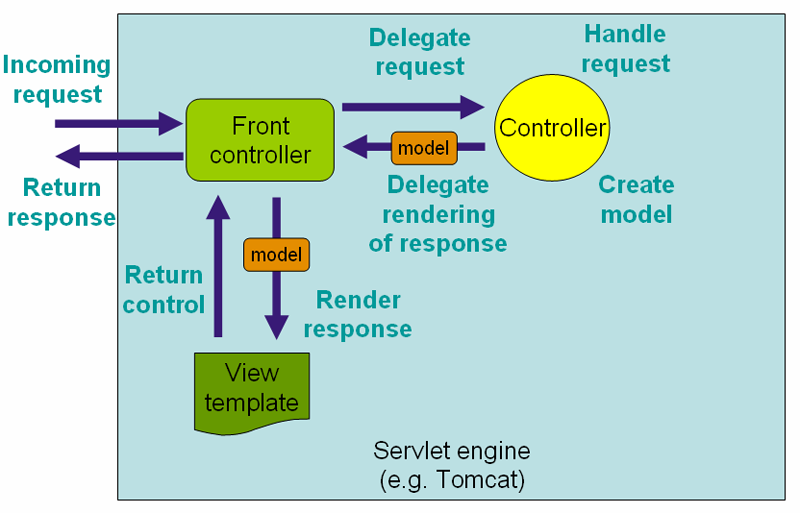
\includegraphics[width=130mm]{images/tourliveweb/springmvc.png}
	\caption{Aufbau von Spring MVC \cite{springsourcemvc2011}}
	\label{fig:springmvc}
\end{figure}

Die Anfragen werden durch den Front Controller empfangen und an den passenden Controller der Applikation weitergeleitet. Dieser fügt die angeforderten Daten (Model) hinzu. Das Model wird dann in die View Templates eingefügt und via den Front Controller an den Client zurückgeschickt.
\\

Dieses abstrakte Vorgehen kann durch ein konkretes Beispiel sehr gut dargestellt werden. Eine Anfrage wird durch den Aufruf einer URL im Browser ausgelöst (z.B. http://www.tourlive.ch/rennen). Der Front Controller sucht den Applikations Controller für die Ressource \textit{/rennen}. Bereitet das Model, in diesem Fall alle sichtbaren Rennen, vor und sendet dieses zurück. Der Front Controller sucht den View Resolver und übergibt das Model (alle sichtbaren Rennen). Dort wird das Model zur Darstellung gebracht und schlussendlich via den Front Controller an den Browser zurückgesendet. Für jede Ressource gibt es also einen Controller, dabei können aber auch generische Elemente wie z.B. der Rennname in der Ressource verwendet werden (z.B. http://www.tourlive.ch/rennen/tourdesuisse).
\\

Für die Einarbeitung in das Spring Framework wurden verschiedene Quellen verwendet. Alle Angaben dazu befinden sich im Literaturverzeichnis. Der obige Abschnitt ist eine Zusammenfassung von Inhalte aus den SpingSource Tutorials \cite{springsourcemvc2011} und Mkyong \cite{springmvcexamples2011} .

\section{Externes Design - Android App}
Folgendes Dokument beschreibt das externe Design der Android App. Als Designgrundlage der Mockups dienen primär die in Zusammenarbeit mit cnlab festgelegten Requirements. Als Referenz stand die bestehende Symbian-App zur Verfügung. 

\subsection{Einführung}
In einem ersten Schritt wurden die Android GUI Principles\footnote{Android GUI Principles\url{http://developer.android.com/design/get-started/principles.html}, zuletzt besuch 21.03.2013}  studiert und aufgrund dieser ein Design-Konzept für die neue App erstellt.
\\

Folgend ein Beispiel einer Applikation, welche den GUI Guidelines entspricht und ähnliche Komponenten benutzt wie die zukünftige TourLiveApp.

\begin{figure}[H]
	\centering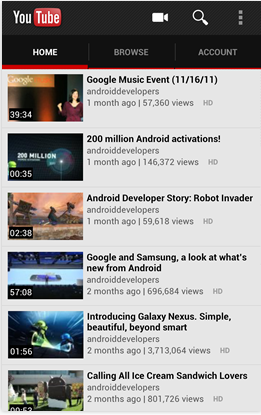
\includegraphics[width=60mm]{images/android/mockups/androidexample.png} 
	\caption{Standard Ansicht nach den Android GUI Guidelines}
\end{figure}

\subsection{Grobübersicht TourLiveApp}
Das Design der Android App gliedert sich grundsätzlich in ein Dashboard sowie 5 Informationsansichten die über Tabs erreichbar sind. Über den "Settings"-Button lassen sich Konfigurationen vornehmen sowie den About Screen anzeigen.

\begin{figure}[H]
	\centering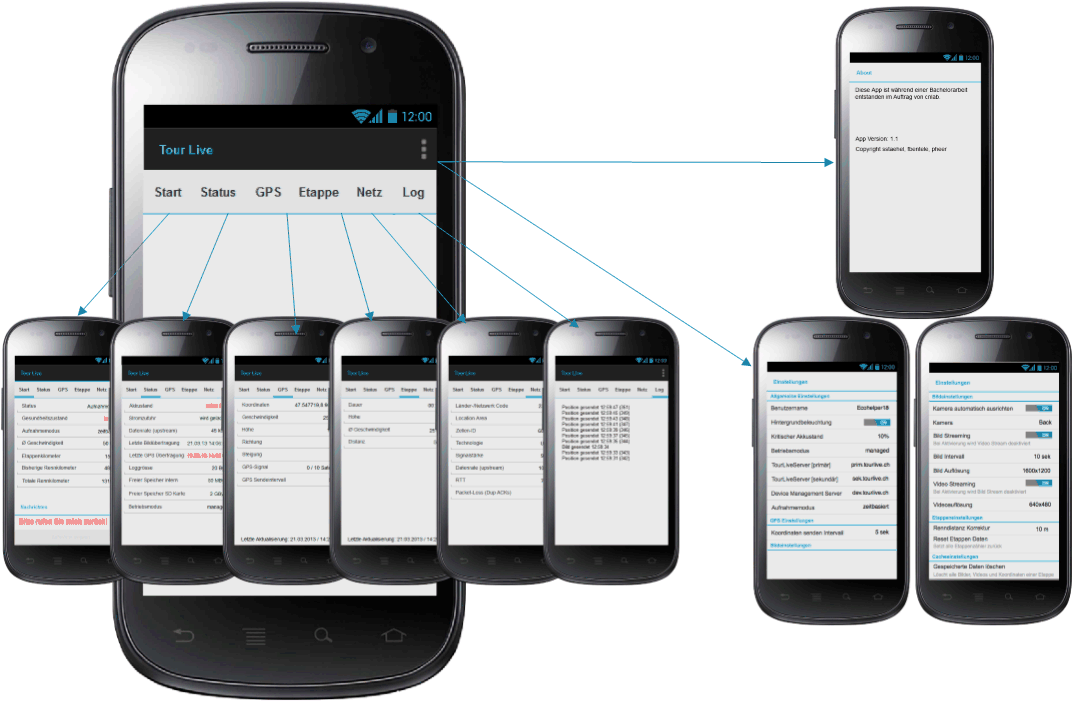
\includegraphics[width=130mm]{images/android/OverviewAndroid.png} 
	\caption{Übersicht über alle Views}
\end{figure}
 
Folgend werden alle Ansichten im Detail beschrieben. Dabei wurde auf mit Hilfe folgender Legende gearbeitet um die einzelnen Werte zu beschreiben:
* 	berechneter Wert der stets aktualisiert wird
+	Wert der aufgrund einer Messung eruiert wird (Android Service Provider)
°	App-Einstellung die angezeigt wird

\subsection{Startscreen - Ansicht}
Wird die App gestartet öffnet sich die „Start“-View. Sie dient als „Dashboard“ und gibt Informationen zum allgemeinen Zustand der App. 

\begin{longtable}{p{5.5cm} p{6.5cm}}
	\raisebox{-\totalheight}{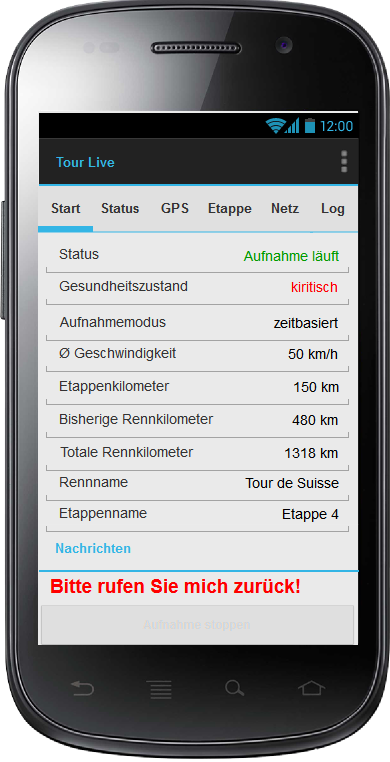
\includegraphics[width=5.5cm]{images/android/mockups/Start.png} }
 & \textbf{Nutzen / Zielperson }\newline

Diese View dient dazu, dem Fahrer und Beifahrer, eine Übersicht zu geben um im Falle eines Problems zu intervenieren. 
Mit Hilfe der Nachrichten kann der Systemüberwacher mit den Autoinsassen kommunizieren kann.\newline
\textbf{Erläuterung der Ansicht} \newline
\textbf{Status:} Zeigt an, ob Daten an den TourLive Server gesendet werden oder nicht \newline
\textbf{Gesundheitszustand:} Zusammenfassung der Ansicht „Status“ \newline
\textbf{Aufnahmemodus (°):} manuell, zeitbasiert, fernverwaltet, externe Stromquelle \newline
\textbf{Durchschnittsgeschwindigkeit (+):} Die Durchschnittlichegeschwindigkeit wird ermittelt, über alle bereits gemessenen Locations, anhand deren Geschwindigkeit \newline
\textbf{Etappenkilometer (*):} Die in der aktuellen Etappe zurückgelegten Kilometer \newline
\textbf{Bisherige Rennkilometer (*):} Die ganze Strecke, über mehrere Etappen verteilt, die zurückgelegt wurde. Dieser Wert wird vom TourLiveServer übermittelt. \newline
\textbf{Totale Rennkilometer (*):} Die totale Anzahl Kilometer, die in diesem Rennen zurückgelegt wird. Wird vom TourLiveServer an die App übermittelt. \newline
\textbf{Nachrichten (*):} Das Management Device Portal hat die Möglichkeit, Nachrichten via das Mobile an die Fahrer zu übermitteln. Diese werden rot dargestellt.\\

\end{longtable}



\subsection{Status - Ansicht}
Allgemeiner Zustand des Systems. Orange eingefärbte Zustände können längerfristig zu Problemen führen, rot eingefärbte Zustände sind kritisch und verhindern das einwandfreie Funktionieren des Systems. Es folgt eine Beschreibung der einzelnen Zustände: 

\begin{longtable}{p{5.5cm} p{6.5cm}}
	\raisebox{-\totalheight}{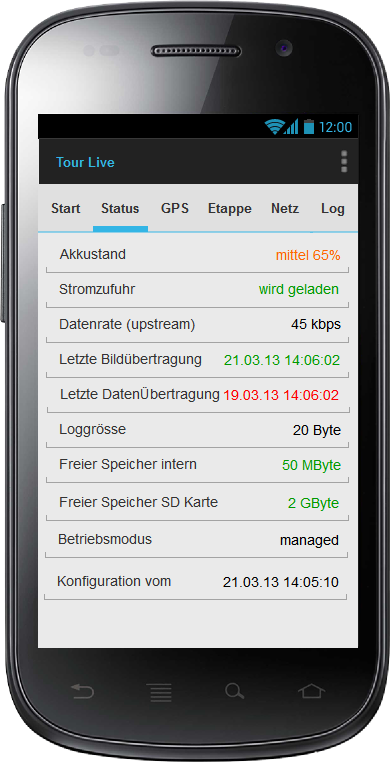
\includegraphics[width=5.5cm]{images/android/mockups/Status.png} }
 & \textbf{Nutzen / Zielperson }\newline

Zielperson ist auch hier der Laie (Fahrer / Beifahrer der auf einen Blick sehen möchte ob die App korrekt funktioniert.  Aus diesem Grund werden problematische Werte orange und kritische Werte rot hinterlegt. \newline
\textbf{Erläuterung der Ansicht} \newline
\textbf{Akkustand (*):} gut (70\% - 100\%, grün), mittel (30\% - 70\%, orange), schwach (0\% - 30\%, rot)\newline
\textbf{Stromzufuhr (*):} nicht vorhanden (rot) / wird geladen (grün)\newline
\textbf{Datenrate (upstream) (*):} Datenrate mit der Daten an den Server übertragen werden.\newline
\textbf{Letzte Bildübertragung (*):} Zeitpunkt der letzten Bildübertragung (< 2min grün, 2min< x <3min orange, >3min rot)\newline
\textbf{Letzte GPS Übertragung:} Zeitpunkt, wann die letzten Positionsdaten übertragen wurden (< 2min grün, 2min< x <3min orange, >3min rot)\newline
\textbf{Loggrösse (*):} Grösse der Logdatei \newline
\textbf{Freier Speicher intern (*):} Nicht belegter Telefonspeicher (50% - 100%, grün, 
30\% - 50\%, orange, 0\% - 30\%, rot) \newline
\textbf{Freier Speicher SD Karte (*):} Freier Platz auf der SD Speicherkarte (50\% - 100\% grün, 30\% - 50\% orange, 0\% - 30\% rot) \newline
\textbf{Betriebsmodus (°):} managed (Gerät wird vom Device Management Portal verwaltet) oder unmanaged (Gerät wird über die lokalen Geräteeinstellungen verwaltet)
\\

\end{longtable}



\subsection{Daten - Ansichten}
Die folgenden Ansichten zeigen alle Informationen, welche an den Server übermittelt werden. Am unteren Rand der Ansicht wird jeweils die „letzte Aktualisierung“ angezeigt. Dies entspricht dem Zeitpunkt wann die Daten zum letzten Mal von den verschiedenen Service Providern bezogen bzw. berechnet und an den TourLiveServer übertragen wurden. Dieser Übertragungsintervall kann in den Einstellungen definiert werden.

\subsubsection{Nutzen / Zielperson}
Diese Ansichten helfen vorrangig dem Techniker allfällige Probleme zu erkennen. Beispielsweise um zu überprüfen ob  die korrekten Werte an den Server übertragen werden.

\subsubsection{GPS – Übersicht}

\begin{longtable}{p{5.5cm} p{6.5cm}}
	\raisebox{-\totalheight}{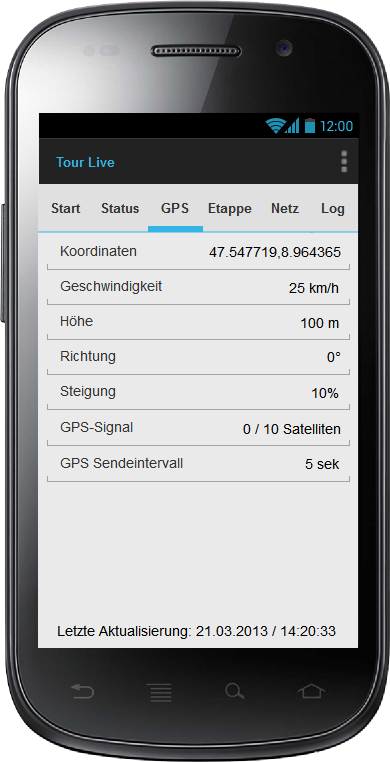
\includegraphics[width=5.5cm]{images/android/mockups/GPS.png} }
 &
\textbf{Erläuterung der Ansicht} \newline
\textbf{Koordinaten (*):} Empfangene GPS Koordinaten im Format WGS84\newline
\textbf{Geschwindigkeit (*):} Empfangene Geschwindigkeit vom Satellit gemessen\newline
\textbf{Höhe (*):} Höhe, vom Satellit ermittelt\newline
\textbf{Richtung (+):} Richtung in Grad, Abweichung von Norden, wichtig um zu erkennen, ob gleich wie die Windrichtung\newline
\textbf{Steigung (+):} Aktuelle Steigung über 100 Meter gemessen\newline
\textbf{GPS-Signal (*):} Verfügbarkeit der GPS-Satelliten\newline
\textbf{GPS-Intervall (°):} In welchem Intervall die GPS-Daten getracked werden. \newline
\textbf{Letzte Aktualisierung (*):} Zeitpunkt, der letzten Aktualisierung der Daten
\\

\end{longtable}

\subsubsection{Etappen – Übersicht}
Alle Informationen rund um die gesammelten Etappendaten.
\begin{longtable}{p{5.5cm} p{6.5cm}}
	\raisebox{-\totalheight}{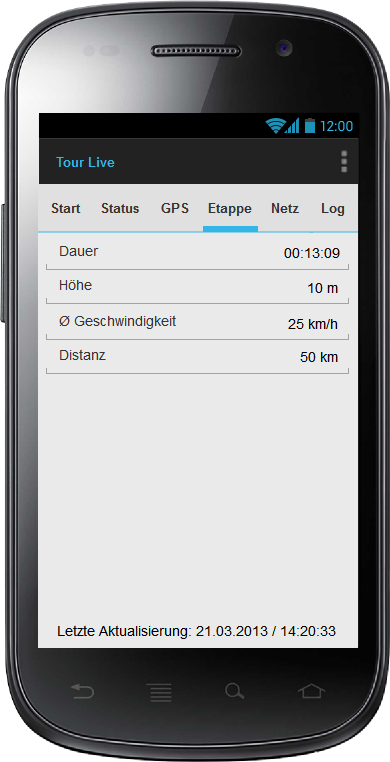
\includegraphics[width=5.5cm]{images/android/mockups/Etappe.png} }
 & 
\textbf{Erläuterung der Ansicht} \newline
\textbf{Dauer (*):} verstrichene Zeit während der aktuellen Etappe seitdem die Aufnahme gestartet wurde.\newline
\textbf{Höhe (*):} zurückgelegte Höhe, berechnet über alle bisher gesammelten Positionsdaten\newline
\textbf{Durchschnittsgeschwindigkeit (*):} Die Durchschnittliche Geschwindigkeit wird über alle der aktuellen Etappe gemessenen Positionsdaten ermittelt. \newline
\textbf{Distanz (*):} Die in der aktuellen Etappe zurückgelegten Kilometer. Wird ebenfalls über sämtliche der aktuellen Etappe ermittelten Positionsdaten berechnet.\newline
\textbf{Letzte Aktualisierung (+):} Zeitpunkt, der letzten Aktualisierung der Ansicht

\\

\end{longtable}


\subsubsection{Netz – Übersicht}
Folgende Ansicht dient zur Eruierung von Übertragungsproblemen. Zur anschliessenden Analyse der Qualität der Datenverbindung werden gleichzeitig zu den Positionsdaten auch Informationen zum vorhandenen Mobilfunknetzwerk gesammelt. 
\begin{longtable}{p{5.5cm} p{6.5cm}}
	\raisebox{-\totalheight}{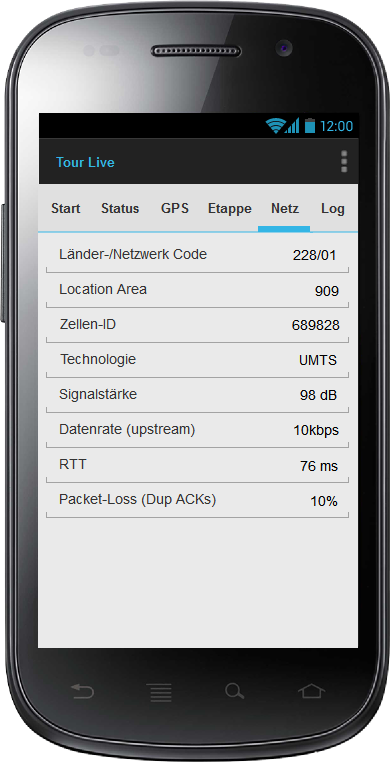
\includegraphics[width=5.5cm]{images/android/mockups/Netz.png} }
 & 
\textbf{Erläuterung der Ansicht} \newline
\textbf{Länder-/Netzwerk Code (+):} Mobile Country\footnote{Mobile Country Code, \url{http://en.wikipedia.org/wiki/Mobile_country_code}, zuletzt besucht 22.03.2013} und Network Codes\footnote{Mobile Network Code, \url{http://en.wikipedia.org/wiki/Mobile_Network_Code},  zuletzt besucht 22.03.2013}  \newline
\textbf{Location Area (+):} Eine Location-Area wird vom Mobilefunkanbieter definiert und fast mehrere Zellen (Antennen) zusammen.\newline
\textbf{Zellen-ID (+):} Zeigt die Zellennummer an mit der das Gerät aktuell verbunden ist.\newline
\textbf{Technologie (+):} Mobiles Kommunikationsprotokoll\newline
\textbf{Signalstärke (+):} Zeigt die aktuelle Mobilfunksignalstärke an\newline
\textbf{Datenrate (upstream) (+):} Gemessene Datenrate bei der Bildübertragung\newline
\textbf{RTT (+):} mit ICMP gemessene Round-Trip-Time\newline
\textbf{Packet-Loss (dup ACKs) (+):} Packetverlust beim Upload der Daten
\\

\end{longtable}




\subsubsection{Log }
Zur Fehlerbehebung allfälliger Fehler werden diverse Aktionen geloggt. 
\begin{longtable}{p{5.5cm} p{6.5cm}}
	\raisebox{-\totalheight}{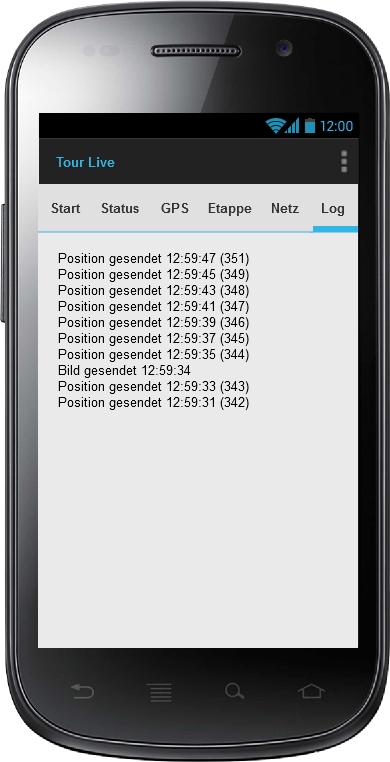
\includegraphics[width=5.5cm]{images/android/mockups/Log.png} }
 & 
Folgende Aktionen werden geloggt:
\begin{itemize}
\item Bild versendet
\item Daten versendet
\item Einstellungen synchronisiert
\item Aufgetrettene Exceptions
\end{itemize}
	

\\

\end{longtable}


\subsection{Einstellungen}
Über den „Settings“-Button in der rechten oberen Ecke werden die App-Einstellungen angepasst. Ist am Geräte ein physischer „Settings“-Knopf vorhanden, können die Einstellungen auch über diesen geöffnet werden.
\subsubsection{Nutzen / Zielperson}
Die Einstellungen werden entweder am Gerät (Betriebsmodus: unmanaged) oder über den DeviceManagementServer (Betriebsmodus: managed) vorgenommen. Die Einstellungen dienen vorgängig technisch versierten Personen um entsprechende Konfigurationen vorzunehmen. 

\begin{longtable}{p{5.5cm} p{6.5cm}}
	\raisebox{-\totalheight}{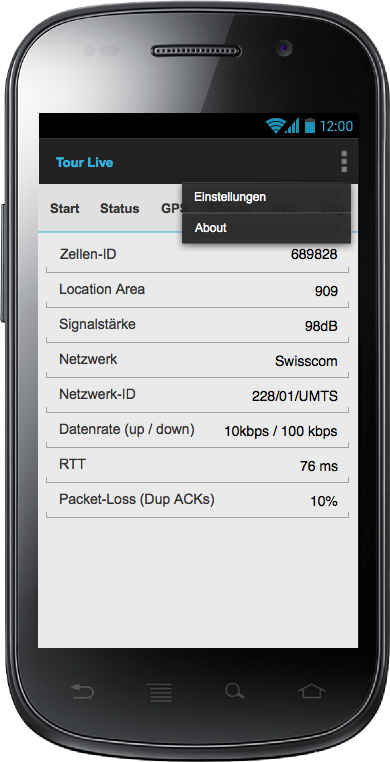
\includegraphics[width=5.5cm]{images/android/mockups/SettingsButtonPressed.png} }
 & 
\textbf{Erläuterung der Ansicht} \newline
\textbf{Einstellungen:} Einstellungen der App \newline
\textbf{About:} Zeigt den About Screen an
\end{longtable}

\begin{longtable}{p{5.5cm} p{6.5cm}}
	\raisebox{-\totalheight}{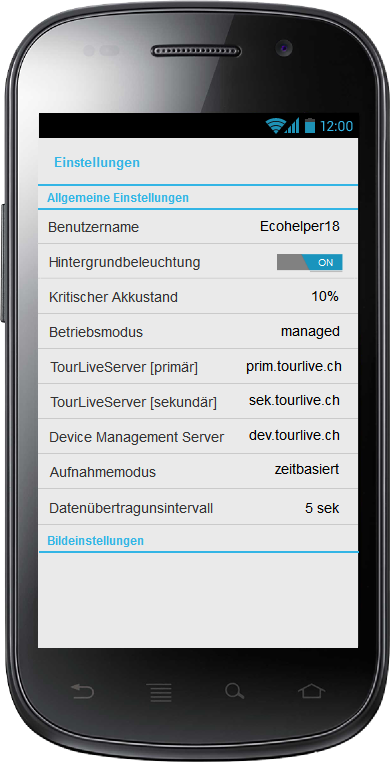
\includegraphics[width=5.5cm]{images/android/mockups/Einstellungen1.png} }
 & 
\textbf{Erläuterung der Ansicht} \newline
\textbf{Benutzername:} Benutzername zur Identifizierung des Gerätes für den Benutzer. Innerhalb des TourLiveSystems wird mit einer eindeutigen Geräteidentifikationsnummer gearbeitet \newline
\textbf{Hintergrundbeleuchtung:} Aktivierung / Deaktivierung der permanenten Hintergrundbeleuchtung  \newline
\textbf{Kritischer Akkustand:} Grenzwert „kritischer“ Akkuzustand für Power-Saving Funktionalität: nach Unterschreiten dieses Wertes werden Stromsparmassnahmen ergriffen \newline
\textbf{Betriebsmodus:} Betriebsmodus „managed“ oder „unmanaged“ \newline
\textbf{TourLiveServer [primär]:} Primärer TourLiveServer an den die Daten gesendet werden \newline
\textbf{TourLiveServer [sekundär]:} Sekundärer TourLiveServer der als Backup dient, falls der primäre TourLiveServer nicht mehr verfügbar ist  \newline
\textbf{Device Management Server:} Device Management Server mit dem die Gerätekonfiguration synchronisiert wird. \newline
\textbf{Aufnahmemodus:} Aufnahmemodus (zeitbasiert, manuell, fernsteuerung, aufgrund aktiver Stromzufuhr) \newline
\textbf{Datenübertragungsintervall:} Zeitintervall in dem die Positionsdaten/Netzwerkdaten aufgezeichnet, an den Server gesendet und die App-Views aktualisiert werden

\end{longtable}


\begin{longtable}{p{5.5cm} p{6.5cm}}
	\raisebox{-\totalheight}{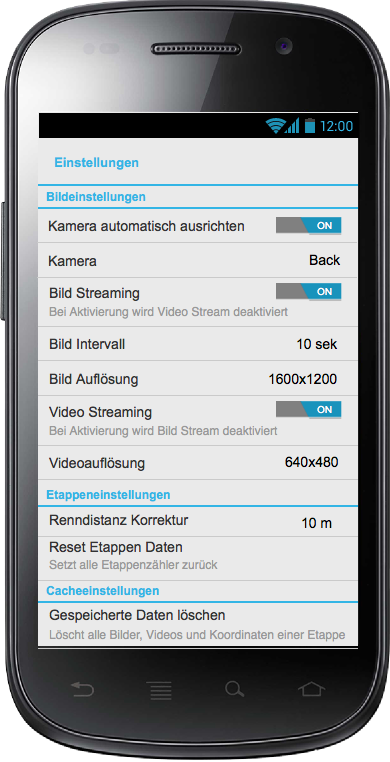
\includegraphics[width=5.5cm]{images/android/mockups/Einstellungen2.png} }
 & 
\textbf{Automatische Ausrichtung der Kamera:} Ist der „Switch“ deaktiviert, so kann über ein Untermenü die Ausrichtung der Kamera explizit definiert werden.\newline
\textbf{Bild- / Video - Streaming:} Aktivierung / Deaktivierung Übertragung von Bildern / Videos (es kann nur Video-Streaming oder Bilder-Streaming aktiv sein) \newline
\textbf{Kamera:} Zeigt die aktuelle Ausrichtung der Kamera an.\newline
\textbf{Bild Intervall:} Zeitintervall in dem die Bilder an den TourLive Server übertragen werden\newline
\textbf{Bild Auflösung:} Auflösung der Bilder (Abhängig vom Gerätetyp)\newline
\textbf{Video Streaming:} Aktivierung / Deaktivierung Übertragung vom Video-Stream (es kann nur Video-Streaming oder Bilder-Streaming aktiv sein)\newline
\textbf{Videoauflösung:} Auflösung des Video-Streams (Abhängig vom Kamera-Modell)

\end{longtable}


\section{Werzeuge und Entwicklungsumgebung}
\label{sec:wekzeugeundentwicklungsumgebung}
Für die drei Teilprojekte TourLive Server, DeviceManagement Server und Aufnahmesystem wurde jeweils die Java Programmiersprache verwendet. Dennoch gibt es Unterschiede bei den Entwicklungsumgebungen, diese sind im folgenden Abschnitt erläutert.

\subsection{TourLive Server}
\begin{itemize}
\item Entwicklungsumgebung: Spring Tool Suite (STS), basierend auf Eclipse, \url{http://www.springsource.org/sts}
\item Framework: Spring MVC, Java Webframework, \url{http://www.springsource.org/}
\item Mockups: Balsamiq Mockup für erste Entwürfe, \url{http://www.balsamiq.com/}
\item Versionierungssystem: git, \url{http://git-scm.com/}
\end{itemize}

\subsubsection{Installation und Deployment}
Um das Projekt zu builden und auf einem Webserver zu betreiben sind folgende Schritte notwendig.

\begin{itemize}
\item Projekt aus GitHub klonen oder komprimierte zip Datei von der CD entpacken
\item In der pom.xml Datei ganz unten ein Profil für die Entwicklungsumgebung erstellen und vergewissern, dass der Datenbankserver läuft
\item Projekt mit Maven builden:
\end{itemize}

\begin{lstlisting}[language=Bash, caption=Build und Test mit Maven]
# bash oder andere Shell starten und
# ins Projektverzeichnis wechseln
~ $> cd RadioTourWebsite

# Dependencies herunterladen und Tests starten
RadioTourWebsite $> mvn install -P meinprofil

# Projekt kompilieren und als deployable war exportieren
RadioTourWebsite $> mvn package -P meinprofil

# Das War File liegt dann im Verzeichnis
RadioTourWebsite $> ~/RadioTourWebsite/target/ba-1.0.0-BUILD-SNAPSHOT.war

\end{lstlisting}

\begin{itemize}
\item Die \textit{war} Datei kann nun auf verschiedene Arten auf dem Tomcat deployed werden, am einfachsten ist das Autodeployment von Tomcat
\end{itemize}
\begin{lstlisting}[language=Bash, caption=Deployment auf Tomcat]
# war Datei aus dem target Ordner in den Tomcat webapps
# Ordner kopieren
RadioTourWebsite $> cp target/ba-1.0.0-BUILD-SNAPSHOT.war /var/lib/tomcat7/webapps/ROOT.war

# Bemerkung: Der Pfad zum webapps Ordner kann sich je
# nach Plattform unterscheiden. Wird die Datei in
# ROOT.war umbenannt so wird die Applikation auf dem
# Domainroot (http://tlng.cnlab.ch/) deployed.
# Danach Tomcat neu starten
RadioTourWebsite $> /etc/init.d/tomcat7 restart

\end{lstlisting}

Sämtliche Videos und Bilder werden nicht direkt über die Webapplikation ausgeliefert, sondern über einen konfigurierbaren Pfad (im Profil ganz unten im pom.xml) abgelegt und von dort aus zur Verfügung gestellt. Der empfohlene Webserver für den Betrieb ist ein Tomcat für die Auslieferung der Bilder und Videodateien kann ein anderer Server verwendet werden, um den Hauptwebserver zu entlasten. Dabei kann aber auch ein Tomcat verwendet werden, die Aussage, dass der Tomcat Server statische Inhalte langsamer ausliefert, wirkt sich gemäss Mark Thomas im Betrieb kaum auf die Performance aus \cite{thomas2010}.

\subsection{DeviceManagement Server}
Java
%TODO Device Management Server beschreiben

\subsection{Aufnahmesystem}
Android Java
%TODO Aufnahmesystem beschreiben

\section{Projektmanagement und weiteres}
Für die Projektplanung und -verwaltung wurde auf verschiedene Hilfsmittel zurückgegriffen. Zum Projektbeginn wurde ein Grobzeitplan erstellt und folgende Meilensteine definiert:

\begin{tabular}{p{2.8cm}p{7.5cm}r}
Meilenstein 0 & Kickoff Meeting & 31.01.2013\\
Meilenstein 1 & Requirements definiert & 15.03.2013\\
Meilenstein 2 & Schnittstellen definiert & 22.03.2013\\
Meilenstein 3 & Erster Prototyp bei Hei präsentiert & 28.03.2013\\
Meilenstein 4 & Erster Feldtest Stäheli & 31.03.2013\\
Meilenstein 5 & Zwischenpräsentation mit Gegenleser und zweiter Prototyp vorgestellt & 26.04.2013\\
Meilenstein 6 & Komplettsystem Test & 02.05.2013\\
Meilenstein 7 & Feature Freeze & 24.05.2013\\
Meilenstein 8 & Code Freeze & 31.05.2013\\
Meilenstein 9 & Abstract/Broschürentext einreichen & 07.06.2013\\
Meilenstein 10 & Abgabe und Präsentation Poster & 14.06.2013\\
\end{tabular}
\\

Die Gesamtplanung mit den An- und Abwesenheiten der Projektmitgliedern und den Meilensteinen wurde in einer Excel Datei erfasst, diese Datei befindet sich auf der CD. Die aufgewendete Arbeitszeit zu den jeweiligen Arbeitspaketen wurde im Projektverwaltungstool Redmine aufgezeichnet und kann unter \url{http://ita.cnlab.ch/redmine/projects/ba-tourlive} eingesehen werden.
\\
%TODO wie machen wir das mit der Zeiterfassung? Redmine? 

\subsection{Testing}
Sämtliche Komponenten wurden kleineren Feldtests unterzogen. Am 6. Juni 2013 konnte das System an den Radsporttagen in Gippingen im realen Rennumfeld getestet werden. Dazu wurde folgender Testbericht erstellt.

\subsubsection{Testbericht Gippingen}
%TODO bitte reviewen und ergänzen / korrigieren
Für den Testlauf an den Radsporttagen in Gippingen wurden drei verschiedene Androidgeräte mit der aktuellsten Version der TourLive App ausgerüstet. Auf dem TourLive Server wurde ein Rennen und eine Etappe erstellt und die Fahrerliste sowie die Marschtabelle importiert. Die drei Aufnahmegeräte wurden dann im RadioTour Wagen bzw. bei zwei weiteren Kommissären im Auto installiert. Zwei zusätzliche Androidgeräte wurden parallel betrieben, jedoch nicht in einem der offiziellen Rennbegleitfahrzeug sondern um weitere Testparameter festzustellen.
\\

Nach wenigen Minuten konnte kein Kontakt mehr zum ersten Aufnahmegerät hergestellt werden. Das Gerät konnte durch die Notfallwiederherstellung per SMS neu gestartet werden, jedoch war nach kurzem Kontakt die Verbindung zum Gerät wieder abgebrochen. Die erste Analyse ergab, dass das Gerät stark überhitzt war und sich deshalb selbst ausschaltete. Ein weiteres Gerät versuchte sich mit dem naheliegenden Deutschen Mobilfunknetz zu verbinden, was aber daran scheiterte, das dass Datenroaming deaktiviert war.
\\

Das dritte Gerät sowie die zusätzlichen Testgeräten hielten den Test durch, obwohl alle Geräte extrem warm geworden sind. Die eingelieferten Daten wurden vom TourLive Server empfangen und verarbeitet. Die Kommunikation zwischen Aufnahmegeräten und Server verlief problemlos.

\subsubsection{Unit Test}
Für den TourLive Server existieren grundlegende JUnit Tests. Diese dienen in erster Linie dazu, die Serverkomponente zu testen und die Entwicklung von weiteren Tests beispielhaft zu dokumentieren.

\subsection{Dokumentation}
Für diese Dokumentation wurde das Textsatzprogramm {\LaTeX} verwendet. Es lässt sich optimal mit dem Versionierungssystem \textit{\gls{git}} kombinieren, was für die Zusammenarbeit an der Dokumentation vorteilhaft ist.
\\

Zu jedem Meeting mit dem Professor wurde ein Protokoll geschrieben. Sämtliche Protokolle und zusätzliche Dokumente befinden sich im Word Format auf der CD.

\section{Plakat}
<<hier kommt das Plakat>>

\section{Kontaktadressen}
\subsubsection{Die Studierenden}

Simon Stäheli\\
Im Langacher 21\\
8805 Richterswil\\
simon@staeheli.me\\

Patrizia Heer\\
Friedbergstrasse 13b\\
8512 Thundorf\\
%TODO nicht-HSR E-Mail Adresse angeben

Florian Bentele\\
Teufener Strasse 113\\
9000 St. Gallen\\
+41 78 883 68 65\\
florian@bentele.me\\

Der betreuende Professor\\
Prof. Dr. Peter Heinzman, cnlab AG\\
Obere Bahnhofstrasse 32b\\
8640 Rapperswil\\
+41 79 243 04 61\\
peter.heinzmann@cnlab.ch\\

Der Industriepartner\\
Lukas Frey, cnlab AG\\
Obere Bahnhofstrasse 32b\\
8640 Rapperswil\\
+41 55 214 33 44\\
lukas.frey@cnlab.ch

\section{Inhaltsverzeichnis der CD}
Auf der beigelegten CD befinden sich folgende Ordner:
%
% 01 Dokumente cnlab
% -- 
% 02 Projektorganisation
% -- 01 Zeitplan.xls
% -- 
% 03 Projektdokumentation
% -- 00 Requirements
% -- 01 Mockups
% -- 02 Domain Model und Diagramme
% -- 03 Sitzungsprotokolle
% -- 04 Zwischenpräsentation
% -- 05 Poster
% 04 Code
% -- 01 TourLive Server
% -- 02 Android Aufnahmesystem
% -- 03 Device Management Server
% -- 04 Recovery App
% 06 Weitere Dokumente
% -- 01 E-Mails
% --
% --

